\documentclass{jarticle}
\usepackage{mathtools, multicol}
\usepackage{color}
\usepackage{url}
\usepackage{comment}
\usepackage{here}
\usepackage{txfonts}
\usepackage{listings, jlisting}
\usepackage{latexsym}
\usepackage{subfigure}

\renewcommand{\lstlistingname}{リスト}

\definecolor{mygray}{rgb}{0.5,0.5,0.5}
\definecolor{purple}{rgb}{1.0,0.4,0.8}
\definecolor{green}{rgb}{0.0,1.0,0.0}

\lstdefinestyle{customplain}{
  belowcaptionskip=1\baselineskip,
  breaklines=true,
  frame=tRBl,
  xleftmargin=\parindent,
  language=,
  showstringspaces=false,
  numbers=left,
  basicstyle=\footnotesize\ttfamily,
  keywordstyle=\bfseries\color{black},
  commentstyle=\itshape\color{black},
  identifierstyle=\color{black},
  stringstyle=\color{black},
}

\lstdefinestyle{customjava}{
  belowcaptionskip=1\baselineskip,
  breaklines=true,
  frame=tRBl,
  xleftmargin=\parindent,
  language=java,
  showstringspaces=false,
  numbers=left,
  basicstyle=\footnotesize\ttfamily,
  keywordstyle=\bfseries\color{purple},
  commentstyle=\itshape\color{green},
  identifierstyle=\color{blue},
}


% 余白の設定
\usepackage[top=20truemm, bottom=16truemm, left=10truemm, right=10truemm]{geometry}

% 図の挿入
\usepackage[dvipdfm]{graphicx}

% より複雑な数学記号
\usepackage{amsmath,amssymb}

% 図の通し番号
\usepackage{subfigure}

\newcommand{\todayd}{%
\the\year.{\ifnum \month < 10 0\the\month \else \the\month \fi}.%
{\ifnum \day < 10 0\the\day \else \the\day \fi}}


\makeatletter

\def\@thesis{人工知能}
\def\id#1{\def\@id{#1}}
\def\department#1{\def\@department{#1}}

\def\@maketitle{
	\begin{center}
		{\huge \@thesis \par} %大きなタイトルが記載される部分
		\vspace{10mm}
		{\LARGE\bf \@title \par} % タイトル部分
		\vspace{20mm}
		{\Large 提出締切: 2013.12.11\par} % 提出年月日部分
		\vspace{5mm}
		{\Large 提出日:  \@date \par} % 提出年月日部分
		\vspace{20mm}
		{\Large \@department \par} % 所属部分
		\vspace{10mm}

		{\Large\@id } % 学籍番号部分
		{\Large \@author} % 氏名 
	\end{center}
\par\vskip 1.5em
}

\makeatother

\title{第4回講義課題 課題番号12}
\date{\todayd}
\department{工学部電子情報工学科}
\id{03-123006}
\author{岩成達哉}


\begin{document}

\begin{titlepage}
	\setlength{\topmargin}{1.1in}
	\vspace{100mm}
	\maketitle
\end{titlepage}


\section{概略}
線画の解釈を行うプログラムをAndroidアプリケーションとして作成した.このアプリケーションでは,2つの方法で入力データを与えることができる.

1つ目は,参考文献\cite{ref:labeling}の平賀先生のページで示されるラベル情報をテキスト入力する方法.2つ目は,与えられた画像を処理して線画の解釈する方法である.

当初の目標は,カメラで撮影した画像に対して処理を行い,線画の解釈を行うというものであったが,写真の解像度に左右され,正しい結果は得られなかった.

一方,図形描画ソフトやパワーポイントなどで作成した画像に対しては,正しい解釈を示せることがわかったため,それらを読み込んで処理するプログラムを作成した.


% -----
\section{作成したプログラムの仕様}
プログラムは,以下の2つの入力方法によって解釈を行う.
\begin{enumerate}
\item 参考文献\cite{ref:labeling}の平賀先生のページで示されるラベル情報をテキスト入力する方法
\item 画像を入力する方法
\end{enumerate}

対応する図形は,参考文献\cite{ref:labeling}にあるように,
\begin{quote}
『対象は3面頂点図形とする。
つまりすべての面が平面(すべての辺が直線)であり、 各頂点には3つの面(したがってその境界として3本の辺)が集まる図形である。』
\end{quote}
ということを前提とする.


\subsection{テキスト入力による解釈}
テキスト入力は,図\ref{fig:labeling}のように頂点を分類し,入力する.これは,参考文献\cite{ref:labeling}に基づく.
\begin{figure}[H]
\begin{center}
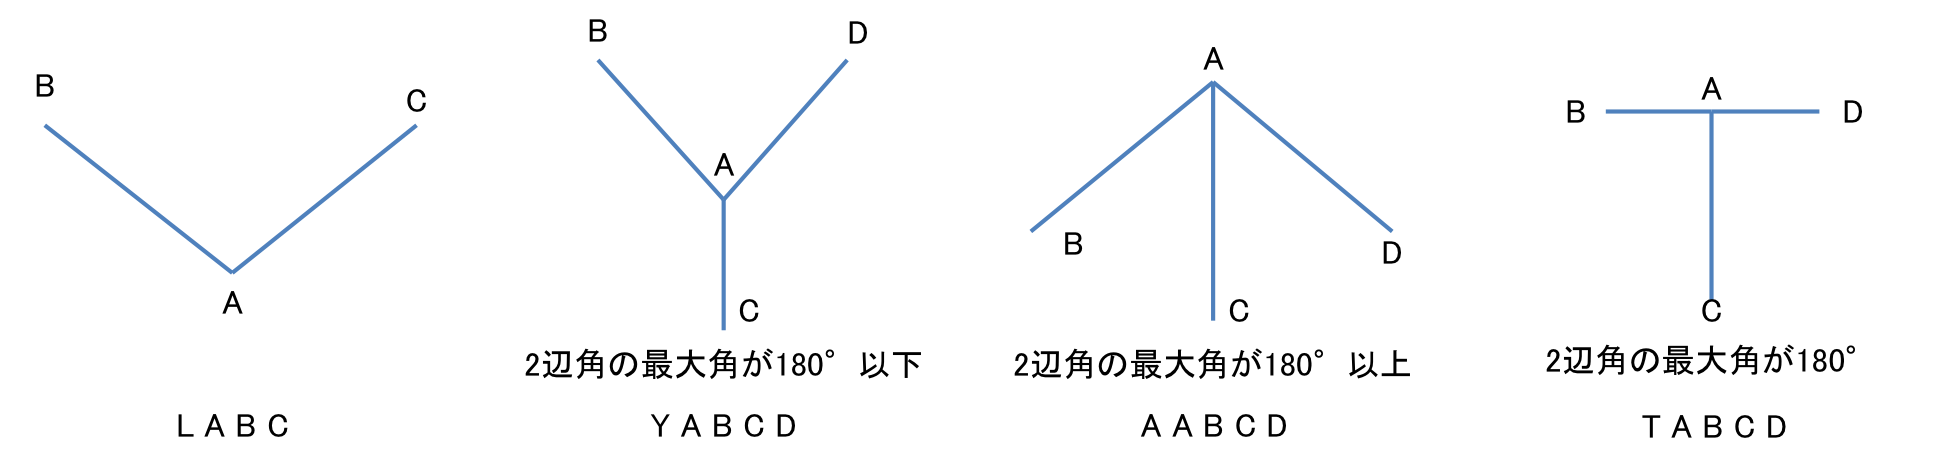
\includegraphics[width=180mm]{image/labeling.png}
\caption{頂点の分類と入力順}
\label{fig:labeling}
\end{center}
\end{figure}

入力は,これらの情報を改行で区切って入力する.また,型の種類はL,A,Y,Tの4つのみであり,頂点の名前は対応さえ正しければ複数の文字でも構わないが,必ず半角スペース1つで区切ることとする.例えば,図\ref{fig:example}のような図形の時は,リスト\ref{code:example}のように入力しなければならない.
\begin{figure}[H]
\begin{center}
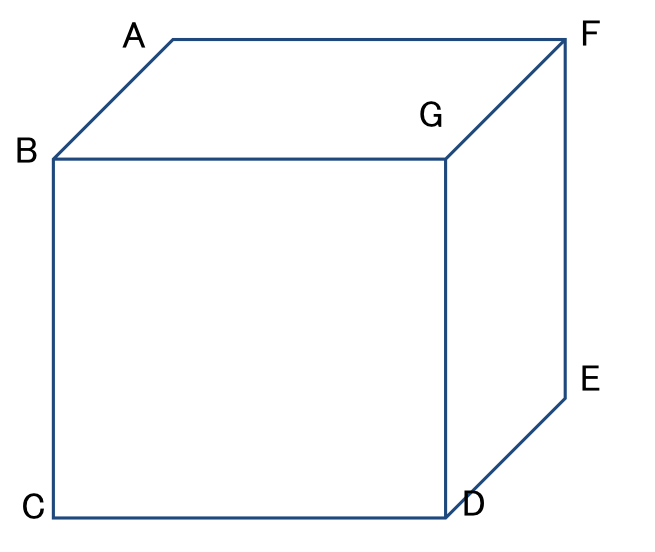
\includegraphics[width=60mm]{image/example.png}
\caption{図形の入力例}
\label{fig:example}
\end{center}
\end{figure}

\lstset{style=customplain}
\lstinputlisting[caption=ラベリング情報の入力例, label=code:example]{source/example.txt}

\textcolor{red}{また,全ての図形は浮いていると判断する.したがって,一番外側の辺は矢印のみ(後述)が候補となる.}これによって,境界を入力することで制約条件を追加することができる.境界の辺は端点を半角スペース区切りで入力し,改行によって分ける.これは,リスト\ref{code:border}のようになる.

\lstset{style=customplain}
\lstinputlisting[caption=境界の入力例, label=code:border]{source/border.txt}





\subsection{画像入力による解釈}
画像を入力することでも解釈を行えるようにした.画像は,jpeg,bitmap,pngに対応しているが,画像の解像度が悪いと解釈が正常にできない.例えば入力データは図\ref{fig:example_image}のような線だけものを入力する.

\begin{figure}[H]
\begin{center}
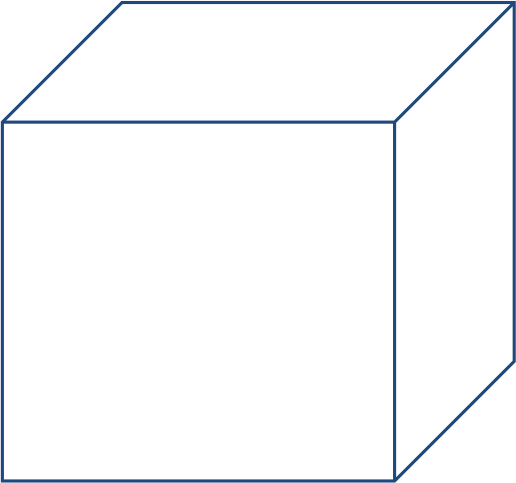
\includegraphics[width=50mm]{image/example_image.png}
\caption{画像の入力例}
\label{fig:example_image}
\end{center}
\end{figure}

カメラで撮影したものは下処理をする必要があるため,画像はカメラで撮影したものと,描画ソフトで描いたもので区別する.

描画ソフトで描いたものを入力すると,前節で示したラベリング情報と境界情報をテキストデータとして出力する.その出力をテキスト入力の場合の解析器と同じものに入力し,解釈を行う.解釈が一意に定まれば,図にその結果を書き込み,定まらない場合は,テキストと図を両方表示する.結果が一意に決まらない場合も,頂点にアルファベットをAから順に振る.

カメラで撮影したものであれば,下処理をして同様の操作を行う.






% -----
\section{実行環境}

\begin{itemize}
	\item Android 2.3以上
	\item OpenCV Manager\cite{ref:opecv_manager}がインストール済み\\
	このインストール方法については,次章に譲る.
	\item 本アプリケーションがインストール済み
\end{itemize}
ただし,実際にテストしたのはAndroid 4.1, 4.2のみである.





% -----
\section{実行の準備}

\subsection{OpenCV Managerのインストール}
今回作成したアプリケーションは,OpenCV\cite{ref:opencv_honke}をライブラリとして用いている.Androidアプリケーションにおいては,OpenCVはライブラリとして完全に独立しており,その主な機能はAndroidアプリケーションとして,個別に用意されている.これが「OpenCV Manager」である.OpenCV Managerは,Play Storeからインストールができる(Play Storeにおいて「OpenCV Manager」と検索するか参考文献のURLから発見できる)\cite{ref:opecv_manager}.Android端末で,検索を行い,インストールを行う.

インストールを行なっていない場合,本アプリケーションをインストールして起動した際に,その旨が表示されPlay Storeへ誘導されるため,インストールボタンを押すことでインストールが出来る.


\subsection{本アプリケーションのインストール}
Play StoreでOpenCV Managerをインストールした後,本アプリケーションをインストールし,実行を行う.

提出したものからの,本アプリケーションのインストールは,「LineArtAnalysis $>$ bin $>$ LineArtAnalysis.apk」というapkファイルによって行う.まず,このapkファイルをAndroid端末にダウンロードする.ダウンロード方法は,DropBox\cite{ref:dropbox}やAndroid FIle Transfer\cite{ref:file_transfer}などを用いることで行う.

ダウンロードしたapkファイルを,File Manager(Androidではアストロファイルマネージャー\cite{ref:astro}などがある)で検索して,クリックすればインストールが始まる.DropBoxなどから直接インストールしてもよい.この際に,設定で「提供元不明のアプリケーションをインストール」にチェックを入れておかなければならない.

以上の内容によって,アプリケーションの実行ができる.


\subsection{本アプリケーションのコンパイル}
本アプリケーションの作成はEclipseによって行っている.開発環境の構築は参考URL\cite{ref:android_dev}によって行える.OpenCVを用いたAndroidアプリケーションの開発は,参考URL\cite{ref:opencv_android}を元に行った.本アプリケーションでは,OpenCVのライブラリをダウンロードし,外部ライブラリとして参照している.

Eclipseでは,アプリケーションは自動でビルドされるため,開発環境が整えられれていれば,自動的に「LineArtAnalysis $>$ bin」フォルダにapkファイルができている.

ソースコードは「LineArtAnalysis$>$src$>$jp$>$narit$>$lineartanalysis」以下のフォルダの内部に,リソースファイルは「LineArtAnalysis$>$res」以下のフォルダの内部にある.





% -----
\section{アプリケーションの使い方}
図\ref{fig:photo}に起動時の画面を示した.

\begin{figure}[H]
\begin{center}
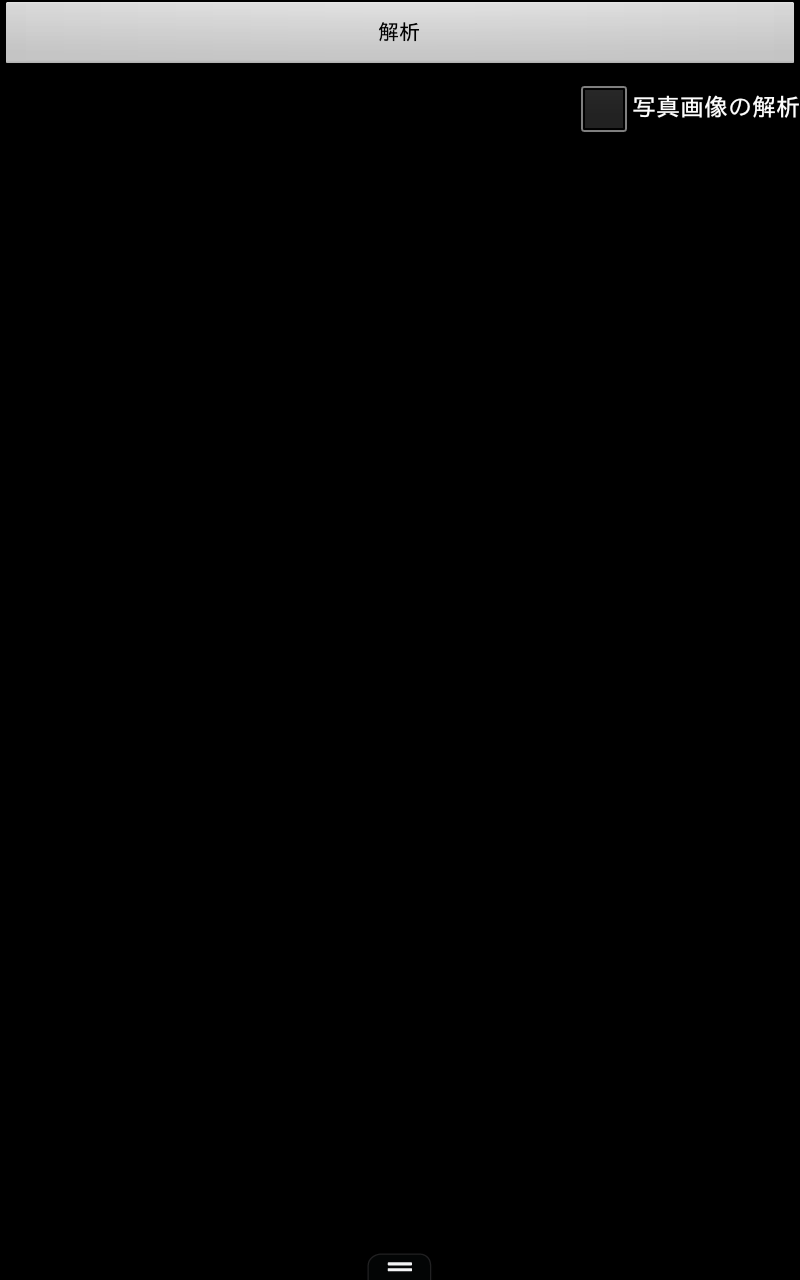
\includegraphics[width=70mm]{../play_store/photo.png}
\caption{起動時の画面}
\label{fig:photo}
\end{center}
\end{figure}


\subsection{画像の解析}
\label{sec:how_to_use_image_analysis}
まずは,画像の解析方法について説明する.図\ref{fig:photo}の上にある「解析」ボタンを押すと,図\ref{fig:file_select}のように端末のファイルエクスプローラが表示される.これは,参考文献\cite{ref:file_explorer}を元に作成した.このエクスプローラを用いて,任意の画像を選択することで,解析させることができる.サンプルとして.「Android/data/jp.narit.lineartanalysis/files」にサンプル画像を7個用意している.

解析の結果は,解釈が一意に定まる場合は画像のみ,一意に定まらなければテキストと画像で表示される.

\textcolor{red}{画像以外のファイルを選択した場合は,アプリがエラー終了する.撮影した写真を入力する場合は,図\ref{fig:photo}の上部にある,「写真画像の解析」をチェックすることで行うが,現在のところ正しい結果は得られていない.}

\begin{figure}[H]
\begin{center}
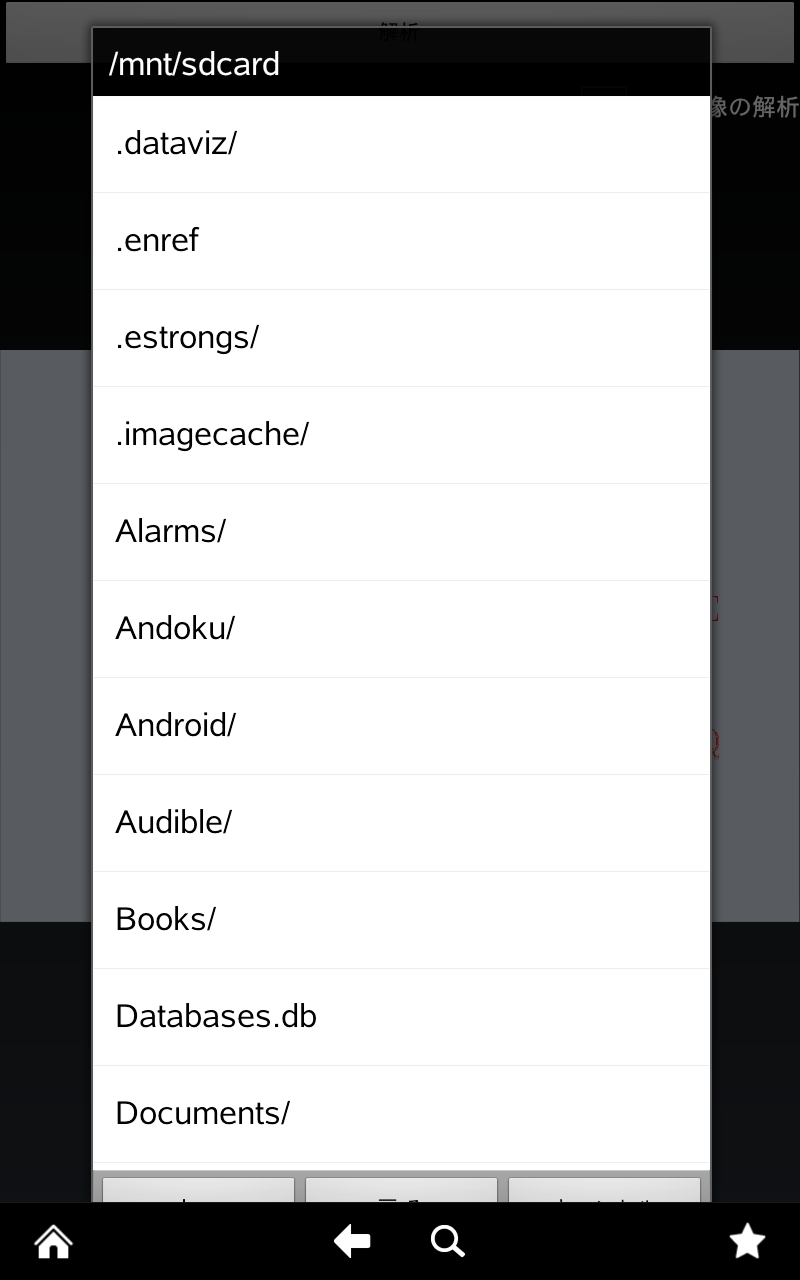
\includegraphics[width=65mm]{../play_store/file_select.png}
\caption{ファイルエクスプローラ}
\label{fig:file_select}
\end{center}
\end{figure}


\subsection{テキストの解析}
次にテキストデータの解析方法について説明する.図\ref{fig:photo}の状態で,Android端末にある「メニュー」ボタンを選択する.このボタンは端末によって,ハードウェアボタンとして実装されている場合もあれば,ソフトウェアボタンとして実装されている場合もある.メニューボタンを押すと,画面の下部に図\ref{fig:menu}が表示される.

\begin{figure}[H]
\begin{center}
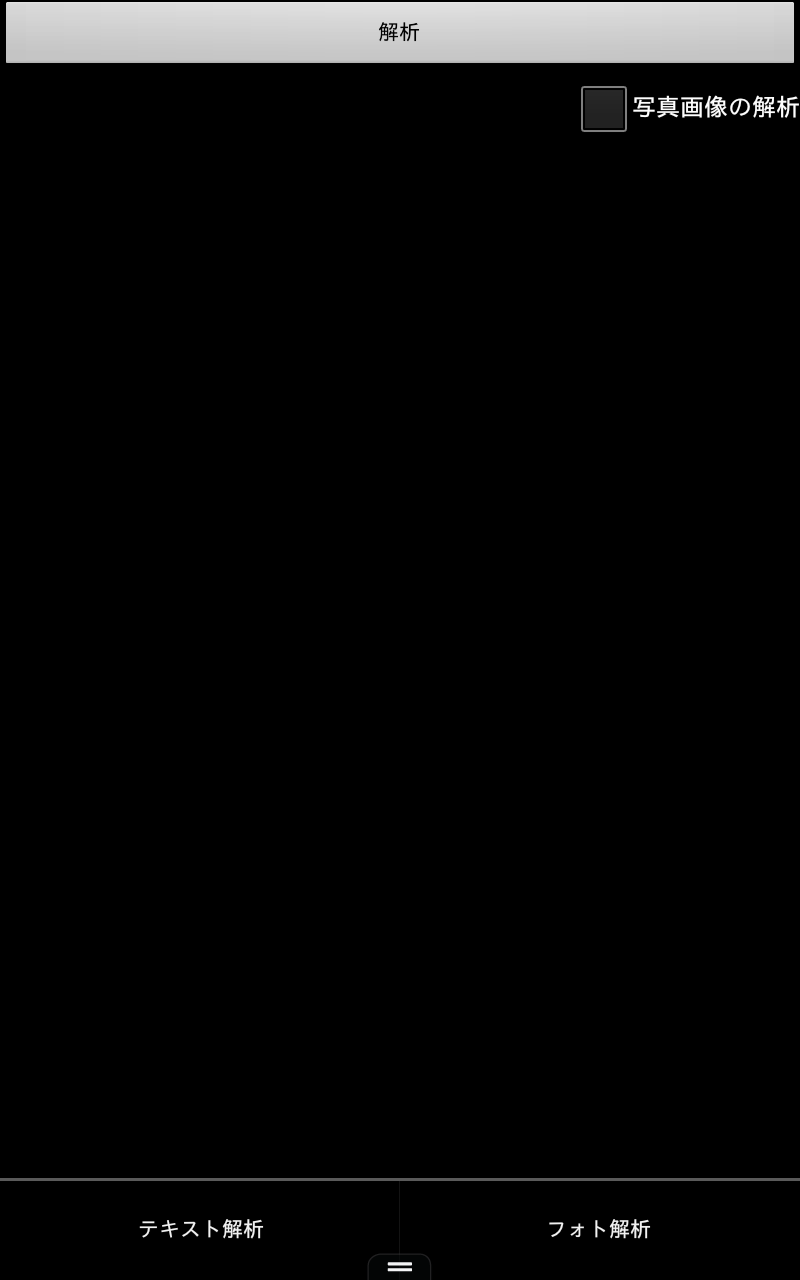
\includegraphics[width=65mm]{../play_store/menu.png}
\caption{メニュー}
\label{fig:menu}
\end{center}
\end{figure}

このメニューの「テキスト解析」を選択すると,図\ref{fig:text}の画面へ移動する.
\begin{figure}[H]
\begin{center}
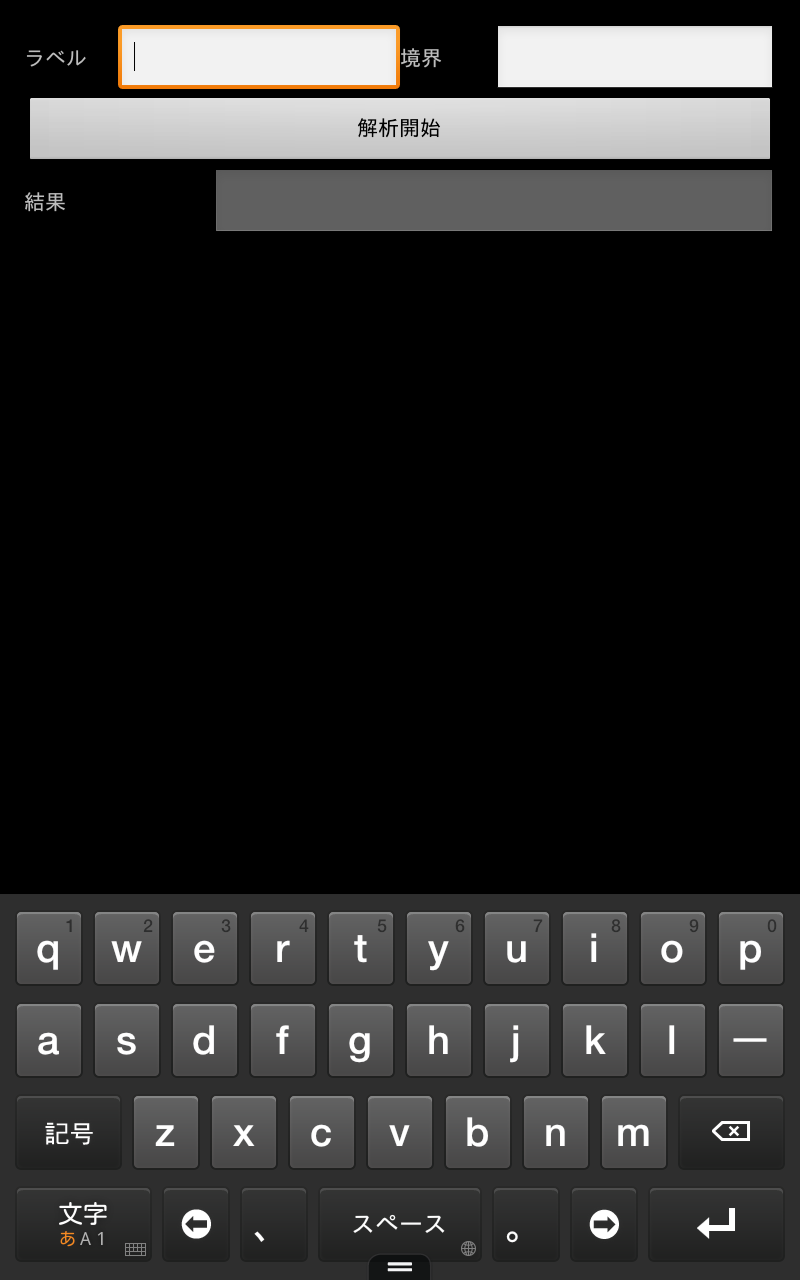
\includegraphics[width=65mm]{../play_store/text.png}
\caption{テキスト解析の画面}
\label{fig:text}
\end{center}
\end{figure}

ここで,ラベル情報と,境界の情報を仕様に従ってそれぞれのテキストビューに入力した後,「解析開始」ボタンを選択すれば,結果が下部のテキストビューに表示される.




% -----
\section{アプリケーションの構成とアルゴリズム\cite{ref:opencv_api}}
アプリケーションの構成を図\ref{fig:composition}に示した.大きく分けてテキストと画像の2つの入力方法がある.
テキストで辺のラベル情報が入力された場合は,Analyzerを通して結果をテキストデータとして出力する.

写真が入力された場合は,まずPreprocessorで下処理をする.下処理をされた画像,あるいは画像描画ソフトなどで作成した図の場合は,Decorderで頂点や辺を解析し,テキストデータとしてAnalyzerへ送る.Analyzerで線画の解釈を行い,解釈が一意に定まれば,Colorerへ結果を入力し,画像に解釈を書き込む.解釈が一意に決まらなければ,テキストデータとして候補を羅列する.
\begin{figure}[H]
\begin{center}
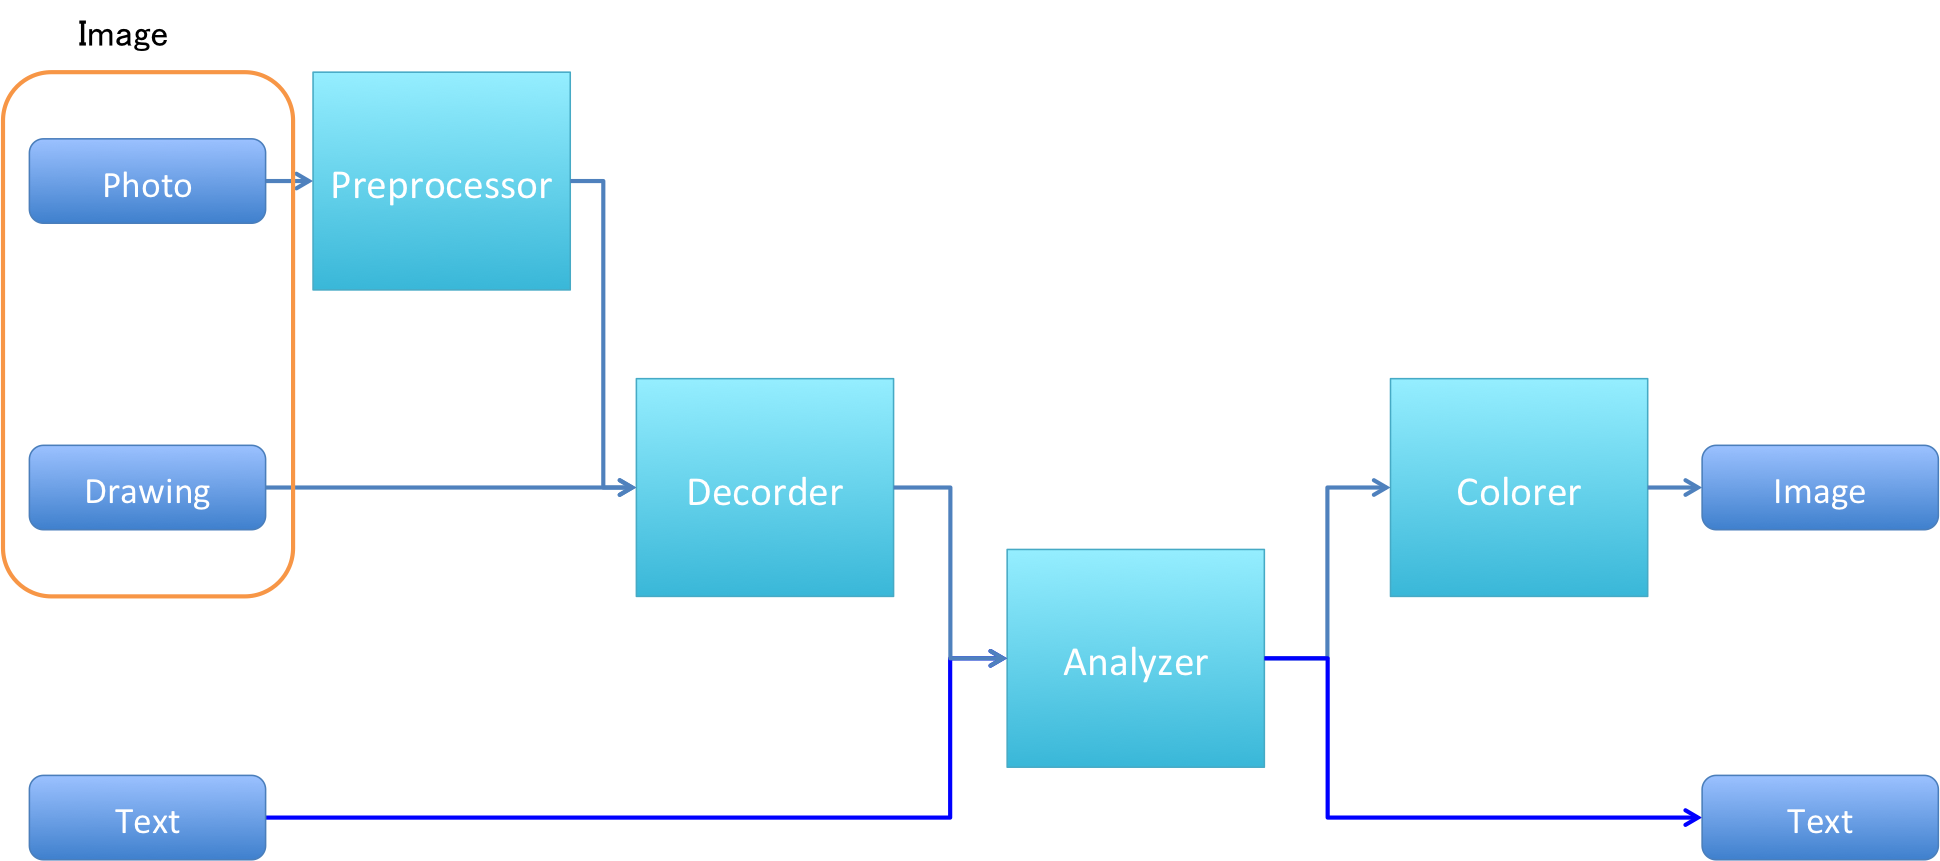
\includegraphics[width=180mm]{image/composition.png}
\caption{アプリケーションの構成図}
\label{fig:composition}
\end{center}
\end{figure}


\subsection{Preprocessor}
写真を入力された時の前処理を行っている.Preprocessorの概要を図\ref{fig:preprocessor}に示した.
\begin{figure}[H]
\begin{center}
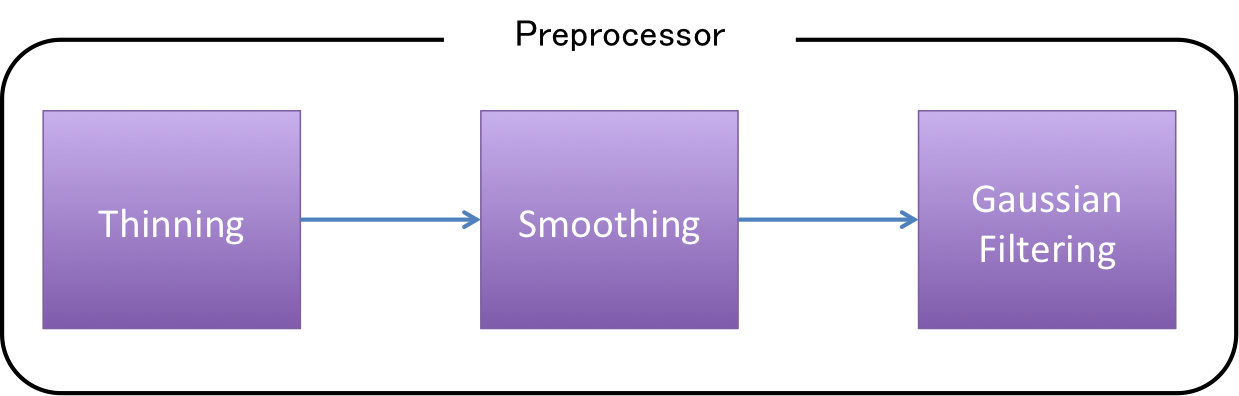
\includegraphics[width=100mm]{image/preprocessor.png}
\caption{Preprocessorの概要}
\label{fig:preprocessor}
\end{center}
\end{figure}


前処理では,まず描かれた線画の細線化を行う.これは,描かれた線に幅がある場合を想定したものである.細線化の処理は,参考URL\cite{ref:thinning}を元に作成した.

細線化を行った画像に対し,さらにsmoothingの処理を施す.つまり,線を滑らかにする処理である.これは,線の歪みやエイリアシングを除くために行った.手法としては,リスト\ref{code:findContours}のOpenCVのfindContours関数を用いて線図の辺を点の集合として取得し,隣り合う点を直線近似して描画するという方法を用いた.
\lstset{style=customjava}
\lstinputlisting[caption=findContours関数, label=code:findContours]{source/findContours.java}

その後,OpenCVのガウシアンフィルタを掛けて,さらに平坦化を行っている.

以上がDecorderの動作である.





\subsection{Decorder}
入力された画像をAnalyzerの入力に合うように,テキストデータとして出力する役を担う.これによって,テキストデータを解釈するときに使うAnalyzerをそのまま用いて線図の解釈が行える.Decorderの構成を図\ref{fig:decorder}に示した.
\begin{figure}[H]
\begin{center}
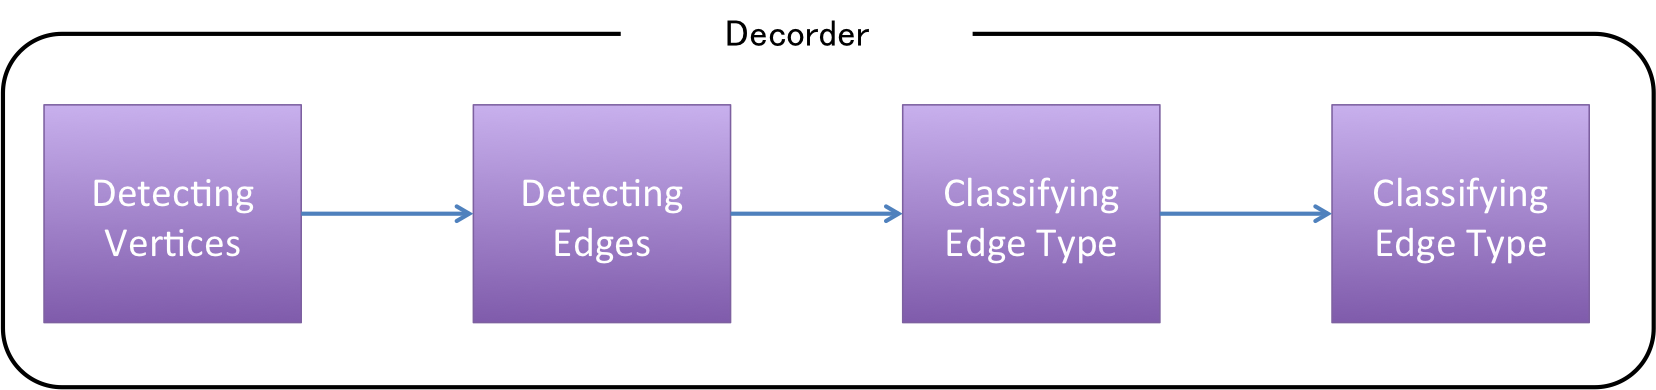
\includegraphics[width=130mm]{image/decorder.png}
\caption{Decorderの概要}
\label{fig:decorder}
\end{center}
\end{figure}


\subsubsection{頂点の取得}
まずは,線画の頂点を取得する必要がある.これは,入力が画像がノイズが少なく,線が細いものであれば,特徴点を抽出するOpenCVのAPIに適切な閾値を与えることで取得できる.用いたAPIは,リスト\ref{code:goodFeaturesToTrack}のgoodFeaturesToTrack関数である.閾値は,実験を通して適切と思われる値に経験から設定した.この際に,写真であればHarris検出器を用いたほうが精度が向上したため,そちらを用いている.
\lstset{style=customjava}
\lstinputlisting[caption=goodFeaturesToTrack関数, label=code:goodFeaturesToTrack]{source/goodFeaturesToTrack.java}




\subsubsection{辺の取得}
次に行うのは,取得したどの頂点とどの頂点が接続しているかを取得することである.まず,リスト\ref{code:findContours}のfindContours関数を用いて線画の境界を抽出する.すると,図\ref{fig:contours}のように,一番外側や,境界が点の集合として取得できる.つまり,findContours関数で得られるのは,「点の集合」のリストである.
\begin{figure}[H]
\begin{center}
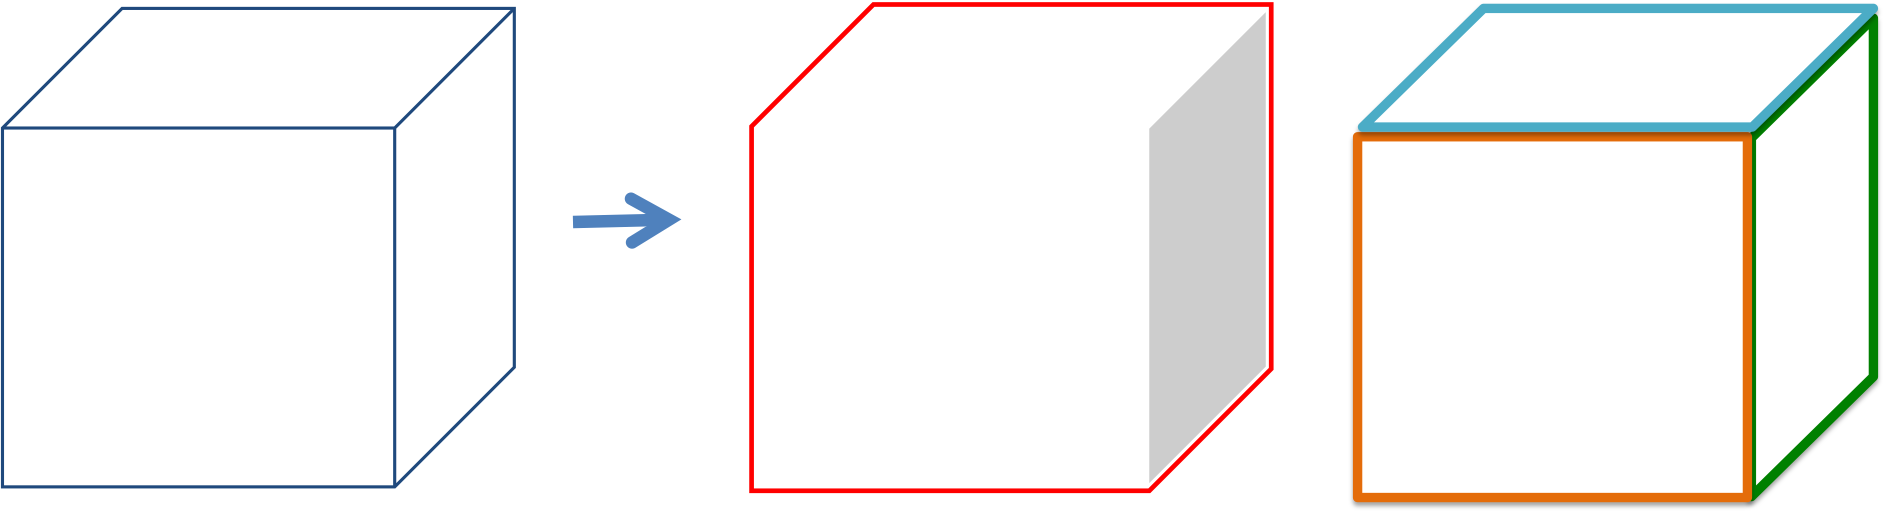
\includegraphics[width=130mm]{image/contours.png}
\caption{境界の様子}
\label{fig:contours}
\end{center}
\end{figure}

これによって,得られたリストを順に探索していき,前節で取得しておいた頂点のどれかと一致した場合は,次にきた頂点との対応を記録する.これがそのまま辺となるのである.厳密には,境界は線画の辺の外側をなぞるように取得されるため,境界の上に頂点は存在しない.そのため,境界に十分近い頂点があれば,辺の上にあると判定している.

また,この際に,一番外側の境界の情報と,頂点情報を元に,外側の境界に属する辺を記録しておくことで,外側の辺をAnalyzerでの制約条件に加えている.

得られた頂点の対応は,後のColorerで用いるために,位置情報を含めて保持しておく.






\subsubsection{辺の分類}
ここまでで,頂点と辺の取得が完了している.問題は,辺の分類である.Analyzerは参考文献\cite{ref:labeling}の平賀先生のページで示されるラベル情報を入力としてとるため,L,Y,A,Tの分類と,頂点の入力順を揃えるという2つを行わなければならない.頂点の分類と入力順を図\ref{fig:labeling}に従う.

まず,頂点の入力順を揃える.これは,構成する3つの頂点を取り出して,それらのベクトルを計算し,2次元の外積を求めることで,どちら向きに並んでいるかを判定することで行う.例えば,図\ref{fig:outer}のように3点A,B,Cがある場合を考える.

\begin{figure}[H]
\begin{center}
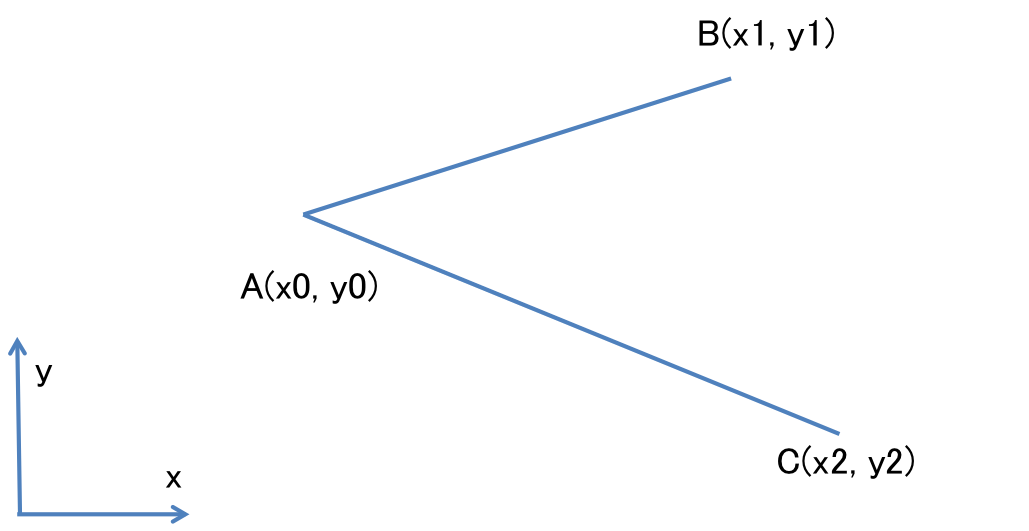
\includegraphics[width=80mm]{image/outer.png}
\caption{2次元の外積}
\label{fig:outer}
\end{center}
\end{figure}

このときは,$\overrightarrow{AB},\overrightarrow{AC}$を求め,それらの外積を以下のように定義する.
\begin{eqnarray}
	\overrightarrow{AB} \times \overrightarrow{AC} &=& (x1 - x0, y1 - y0) \times (x2 - x0, y2 - y0) \nonumber \\
	&=& (x1 - x0) * (y2 - y0) - (y1 - y0) * (x2 - x0)
\end{eqnarray}
こうすると,辺ABと辺ACが図\ref{fig:outer}のようなときに外積が正,辺ABと辺ACが逆の位置関係にあるときに負,辺ABと辺ACが一直線状になる場合は$0$となる.ただし,これは,図\ref{fig:outer}のように,上向きが$y$座標となっている場合である.OpenCVでは,$y$軸が下方向を向くため,符号を反対にして考える.以上を用いて,頂点の順番を図\ref{fig:labeling}に従うように並び替えた.

次は,L,Y,A,Tの分類である.まず,L型は,構成する辺が2つしかない.よって,それをそのまま条件として判定を行えば良い.

一方,辺の数が3つとなった時は,Y,A,Tの分類が必要となる.これは,すでに頂点の並べ替えが終わっているために比較的容易にできる.求めたいのは,図\ref{fig:classifying}の辺ACを含まない方向の$\angle{BAD}$の大きさである.

\begin{figure}[H]
\begin{center}
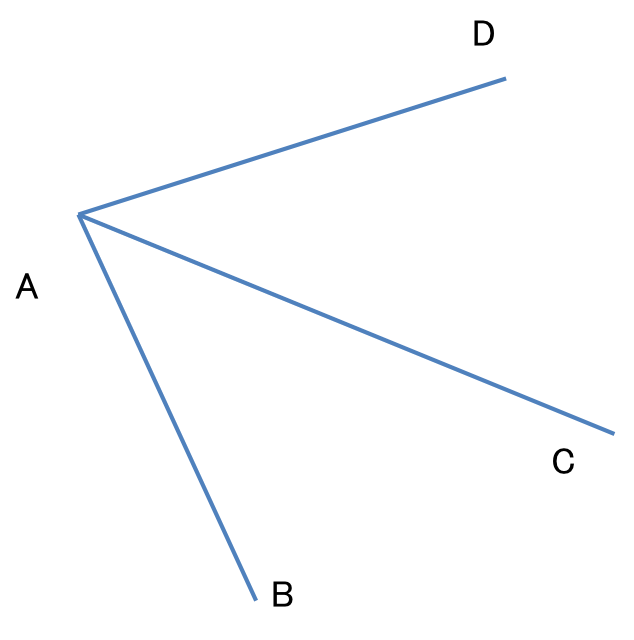
\includegraphics[width=50mm]{image/classifying.png}
\caption{Y,A,Tの分類}
\label{fig:classifying}
\end{center}
\end{figure}

ポイントは,ここまでの処理で,図のように辺が並んでいることである.これを利用すれば,辺ABと辺AC,辺ACと辺ADの間の角をそれぞれ求めて和を取り,360°($2 \pi$)から引けば結果が求まることがわかる.$\overrightarrow{AB} = (x0, y0), \overrightarrow{AC} = (x1, y1) $とすると,辺ABと辺ACの間の角$\theta$は,以下の式で求められる.
\begin{eqnarray}
	 \theta = \arccos {\frac{\overrightarrow{AB} \times \overrightarrow{AC}}{|\overrightarrow{AB}||\overrightarrow{AC}|}} \\
	 ただし,0 \le \theta \le \pi \nonumber
\end{eqnarray}

これによって,Y型やT型でも最大角が求まり,分類が行える.

また,辺の数が1つあるいは4つ以上の時は,今回のアルゴリズムでは判定できないか,不可能図形である.よって,その場合はそれを通知する.


最後に,これらを図\ref{fig:labeling}で示したようなテキスト情報に変換し,Analyzerに入力する.以上がDecorderの動作である.





% -----
\subsection{Analyzer}
Analyzerは,入力されたテキストデータを元に解釈を行う.入力されるデータは,
\begin{enumerate}
\item 図\ref{fig:labeling}のようなラベリング情報
\item 最も外側の辺の集合
\end{enumerate}
の2つである.

\subsubsection{頂点と辺の登録}
まずは,ラベリング情報から,頂点の集合を用意する.頂点は,図\ref{fig:labeling}のように入力が与えられたとき,2つ目にくるもののみ集合に加える.例えば,「L A B C」と与えられた時は,Aを保存する.これを以降では「基準点」ということにする.基準点に対して,入力の1つ目の引数によって,L,Y,A,Tの型が当てはめられる.初めは,その型でありうる全てのラベルを,対応する頂点に与える.ラベルは図\ref{fig:reference}のようになっている.

\begin{figure}[H]
\begin{center}
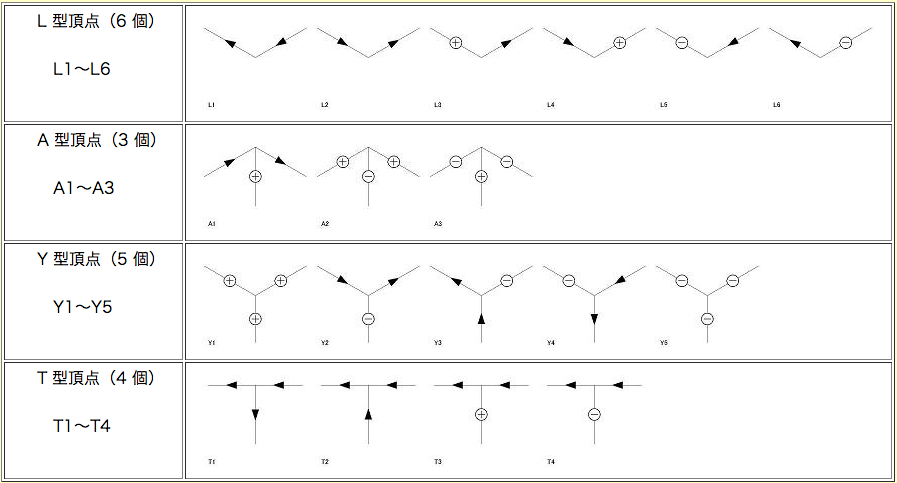
\includegraphics[width=180mm]{image/reference.png}
\caption{L,Y,A,Tのさらなる分類とラベル(\cite{ref:labeling}より引用)}
\label{fig:reference}
\end{center}
\end{figure}

以上で,基準点の集合が形成される.

次に,辺の集合を用意する.辺の集合は,入力の引数の2番目の基準点と,3番目以降の頂点を対応付けることで行う.例えば,「L A B C」と与えられたときは,辺AB,辺ACの2つを集合に加える.この際,すでに同じ辺(辺ABと辺BAは同じと見なす)があれば,集合に登録しない.辺も初めは,$+, -, \rightarrow, \leftarrow$($\rightarrow$は基準点から他の頂点の方向,$\leftarrow$は他の頂点から基準点への方向)の4つのラベルすべてを候補として与えておく.

次に,最も外側の辺の集合の情報が与えられた場合は,それらの辺の候補を$<-,->$の2つに絞る.例えば,「A B(改行)C D」と与えられた場合は,辺ABと辺CDは外側の辺として,候補を減らすことができる.

以上で,基準点と辺の情報を入力データから全て抽出できたことになる.


\subsubsection{候補の決定}
次は,候補の決定,つまり線画の解釈である.これは,前節で用意した基準点の集合と辺の集合の条件を見比べて,候補を絞っていくことで行う.具体的な流れは以下のとおりである.
\begin{enumerate}
\item 基準点の集合に対して,それぞれの基準点に接続している辺のラベルで,基準点の型に当てはまらないものは削除する\\
	例えば,基準点AがT型であり,頂点A,B,C,Dの順で構成されているとする.このとき,辺ABは,図\ref{fig:reference}より,左向きの矢印のみ当てはまるから,他の候補($+, -, \rightarrow$)は削除される.同様に,辺ADも,左向きの矢印のみ当てはまる.
\item 反対に,基準点に接続している辺のラベルを見て,当てはまらない型を基準点の候補から削除する\\
	例えば,基準点AがT型であり,頂点A,B,C,Dの順で構成されているとする.このとき,辺ACの候補が$+,-$のいずれかであれば,図\ref{fig:reference}より,T1,T2は基準点Aの型の候補から削除される.
\item 以上を更新がなくなるまで繰り返す
\end{enumerate}

これによって,それぞれの辺が接続している2つの基準点の制約によって,少しずつ候補が絞られていき,削除が全く行われなくなった時点で終了する.このように,制約が伝播していくアルゴリズムを制約伝播アルゴリズムという.

全ての辺に対して,候補が一つに絞られていればそれが解となり,どれか一つの辺でも複数の解があれば更なる探索が必要であり,どれか一つでも候補がなくなってしまえば不可能図形である.よって,結果は辺の集合が保持している.テキストとして結果を出力する場合は,全ての辺の候補を辺の集合に列挙させれば良い.

以上がAnalyzerの動作である.



\subsection{Colorer}
画像が入力され,候補が一つに絞られる場合は,画像に結果を書き込んで見やすくする役割を持つのがColorerである.そのアルゴリズムは単純で,Decorderから出力された端点の位置座標をもつ辺の集合と,Analyzerから出力された候補を保持した辺の集合を見比べることで行える.

まず,Analyzerからの辺の集合を見て,それに相当する辺をDecorderからの辺の集合から取り出す.辺の候補が$+, -$のいずれかの場合は,2つの端点の中点にその文字を書き出す.一方,矢印の場合は,2つの端点の中点から,適切な方向に適切な長さの辺を2つ描くことで矢印を描く.

以上がColorerの動作である.





%------
\section{実験方法}
アプリケーションの実験を行った.

\subsection{テキスト入力による実験}
まず,テキスト入力に依る実験を行った.これは,図\ref{fig:example}を想定し,リスト\ref{code:example},リスト\ref{code:border}を入力することで行った.

また,テキスト入力による実験は,画像に依る入力の実験と同じ解析器を用いるため,画像に依る入力の実験で正しく動作していることは確認できた.

\subsection{描画ソフトによる画像の入力に依る実験}
描画ソフトで作成した画像を入力して解析を行った.入力した画像は図\ref{fig:input}に示した.いずれもパワーポイントで作成し,ノイズが少なく,線が1ptの幅を持つ図形である.図\ref{fig:sample2}は少しノイズのある図形を上部に配置している.これらは全て,\ref{sec:how_to_use_image_analysis}節で触れたサンプル画像であり,アプリをインストールした際に組み込まれている.


\begin{figure}[H]
\centering
	\subfigure[sample0]{
		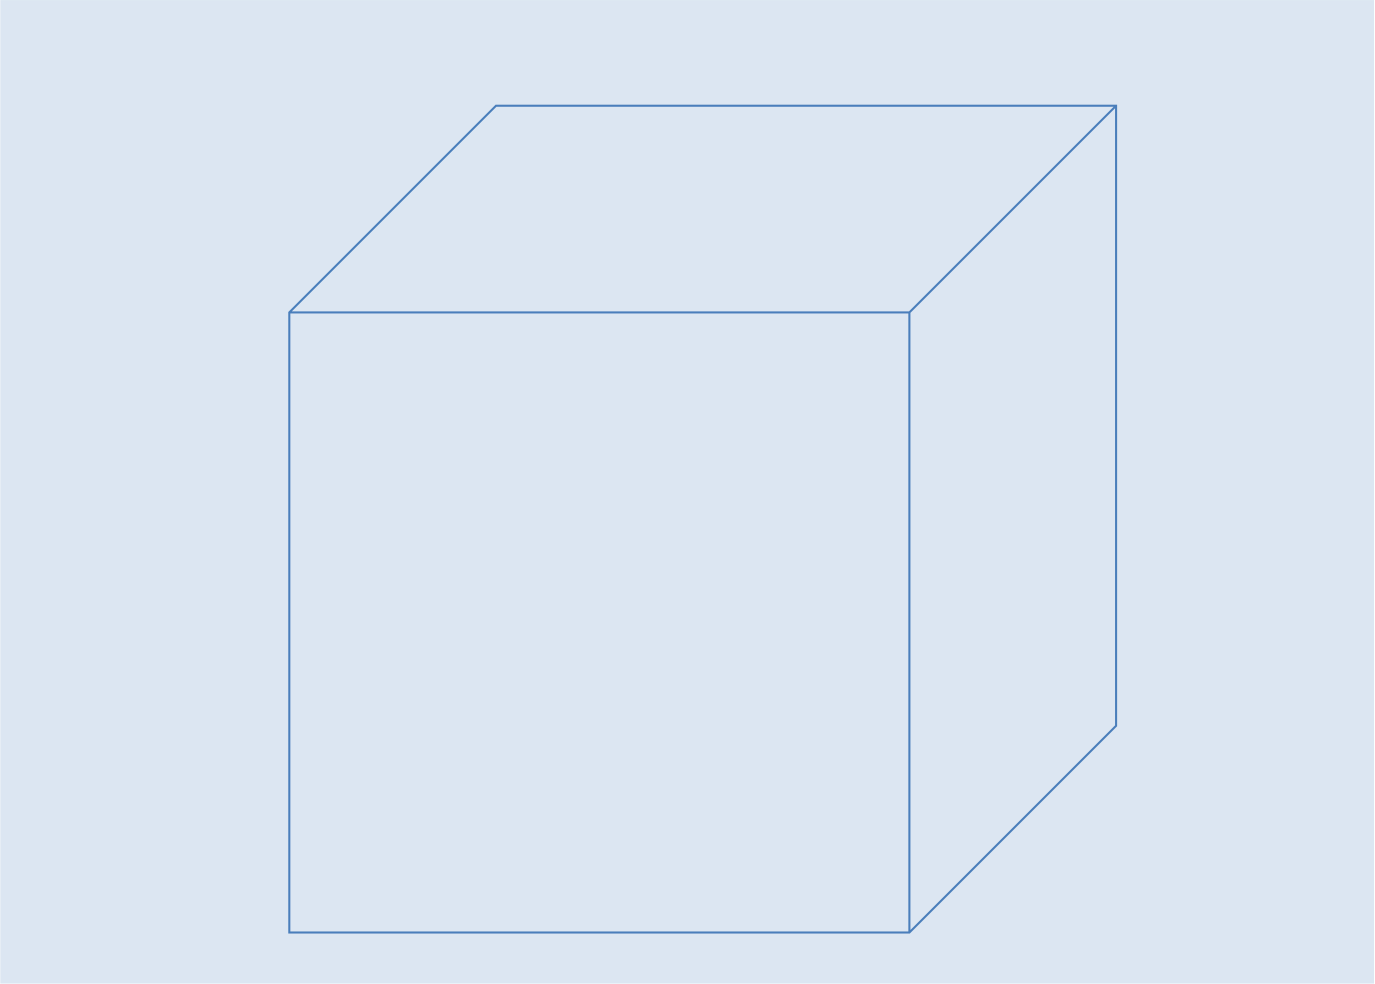
\includegraphics[width=60mm]{../image/sample0.png}
		\label{fig:sample0}}
	\subfigure[sample1]{
		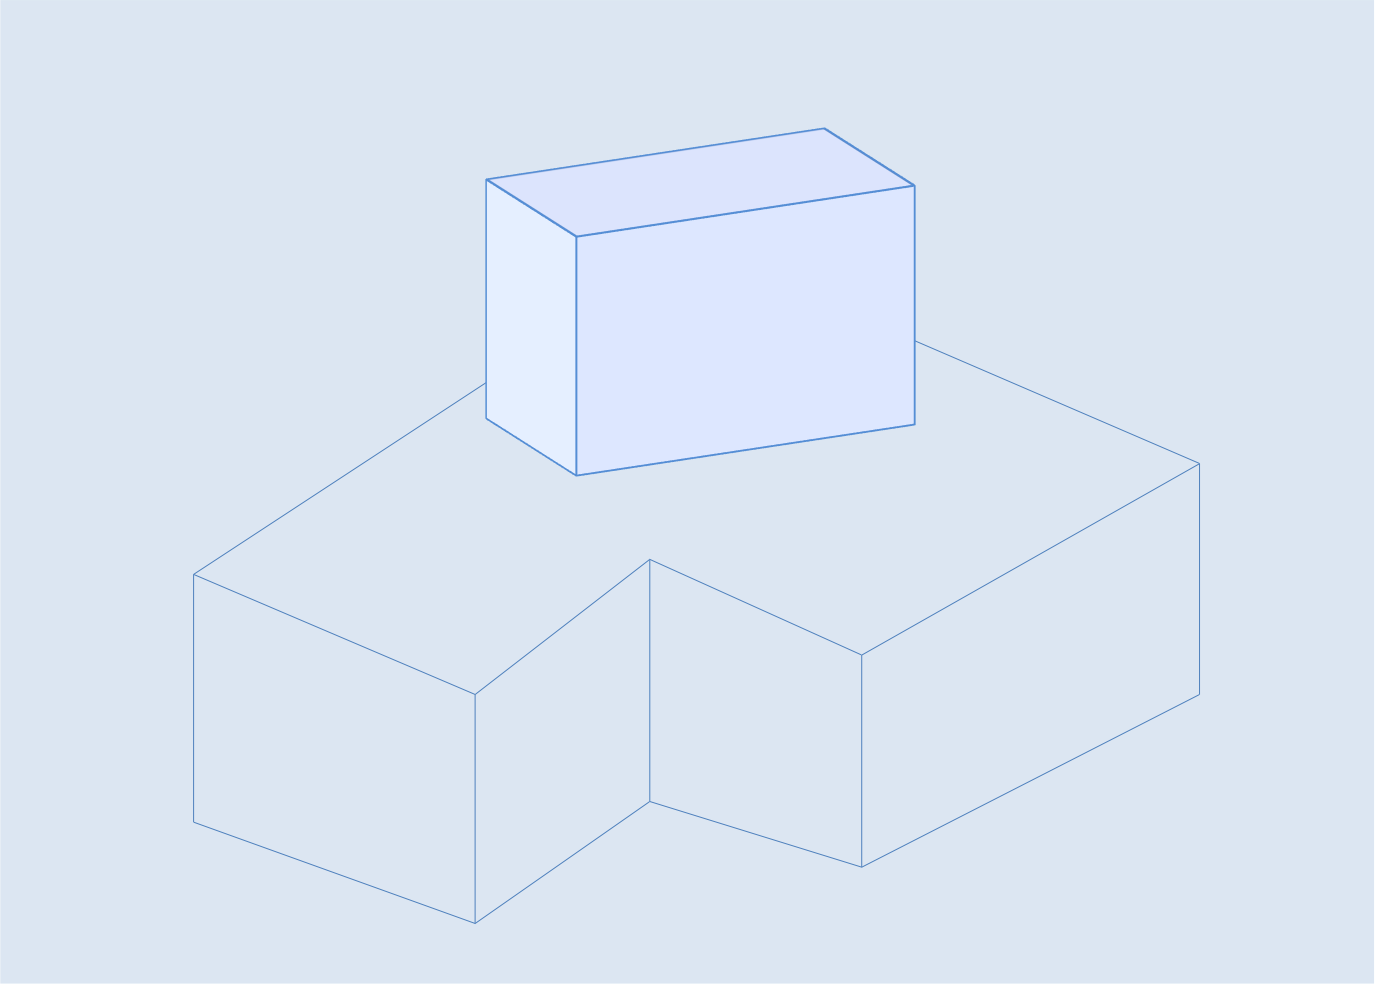
\includegraphics[width=60mm]{../image/sample2.png}
		\label{fig:sample1}}
	\subfigure[sample2]{
		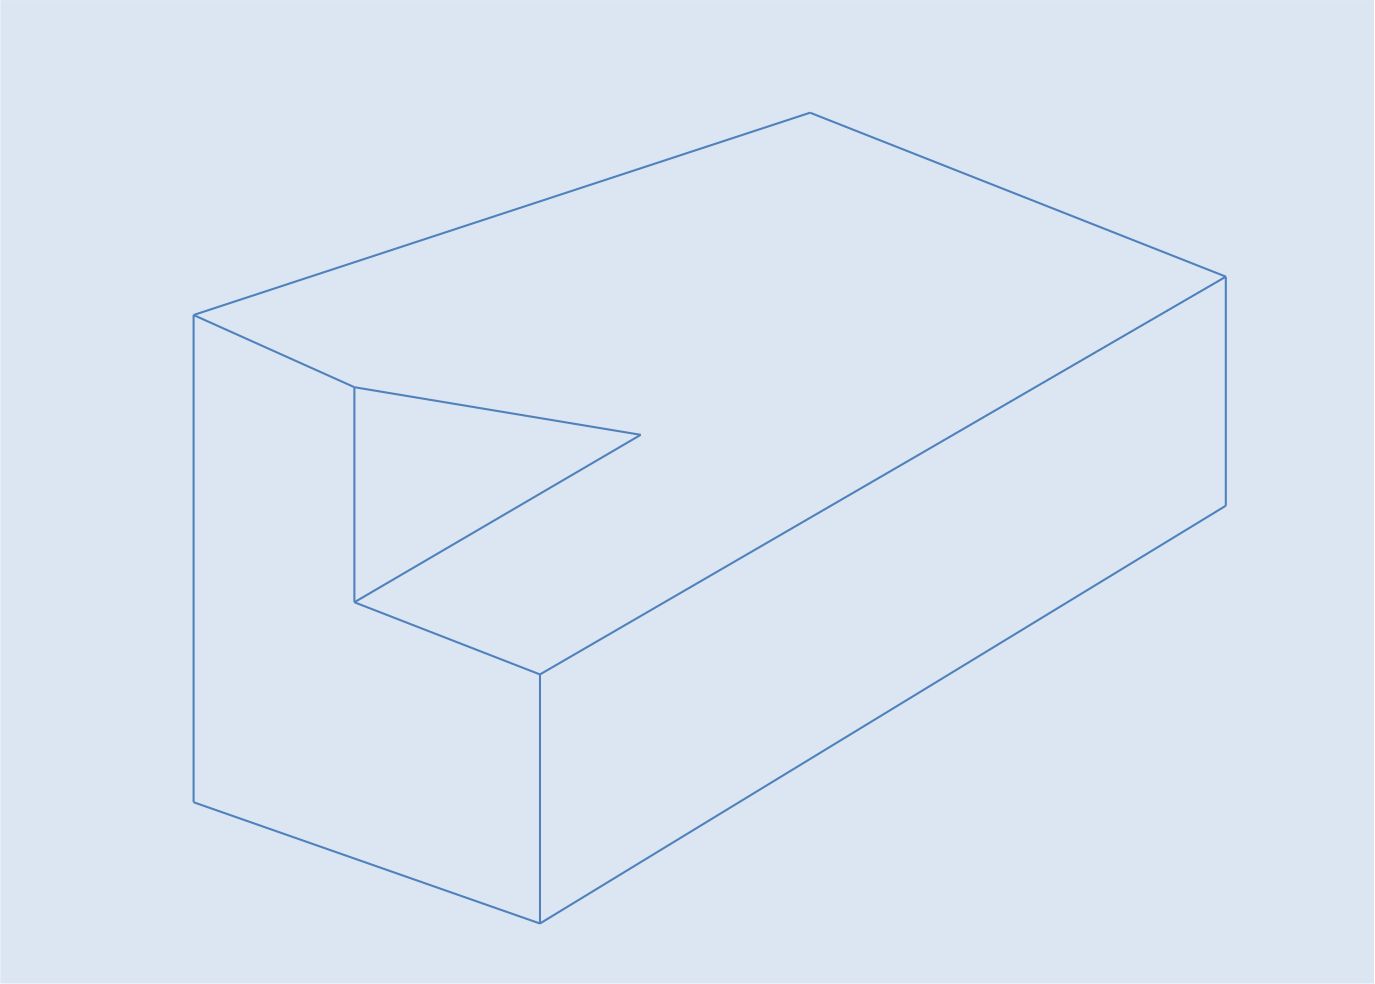
\includegraphics[width=60mm]{../image/sample3.png}
		\label{fig:sample2}}
	\subfigure[sample3]{
		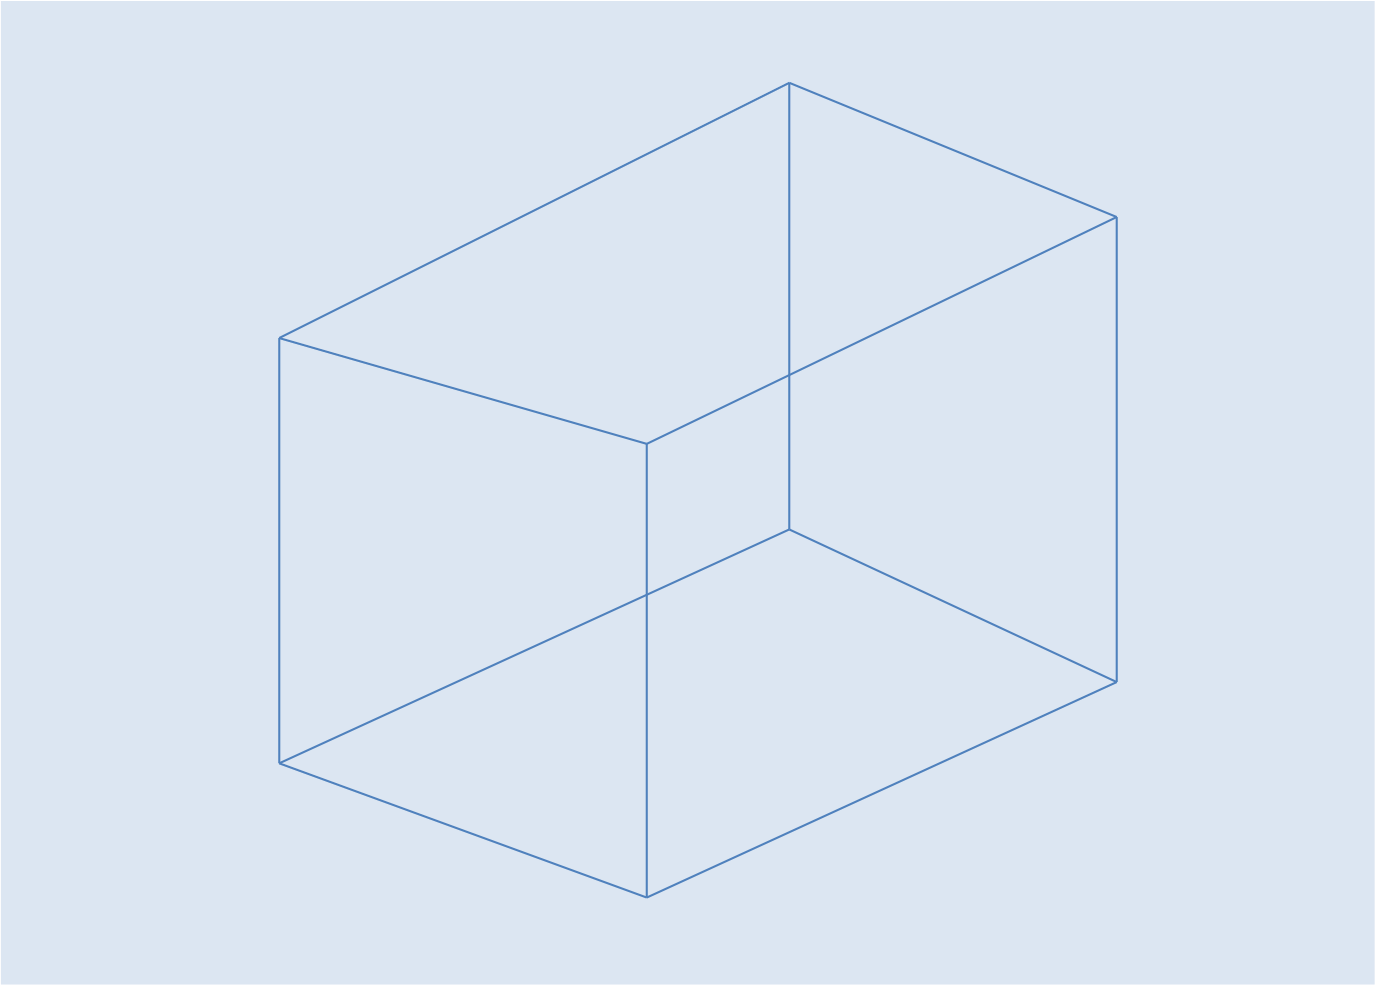
\includegraphics[width=60mm]{../image/sample4.png}
		\label{fig:sample3}}
	\subfigure[sample4]{
		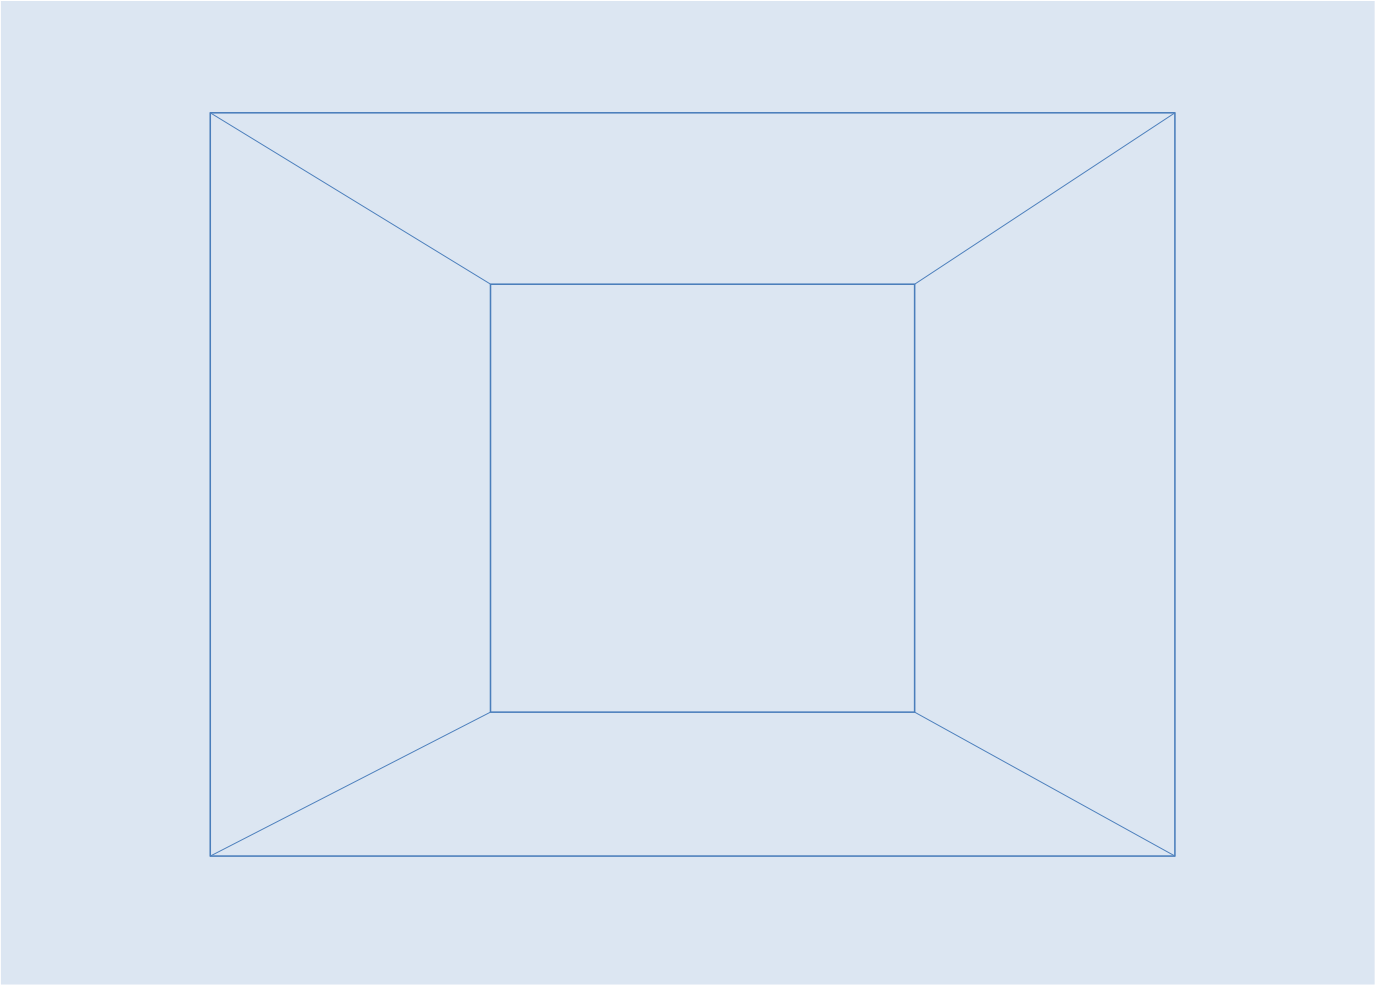
\includegraphics[width=60mm]{../image/sample5.png}
		\label{fig:sample4}}
	\subfigure[sample5]{
		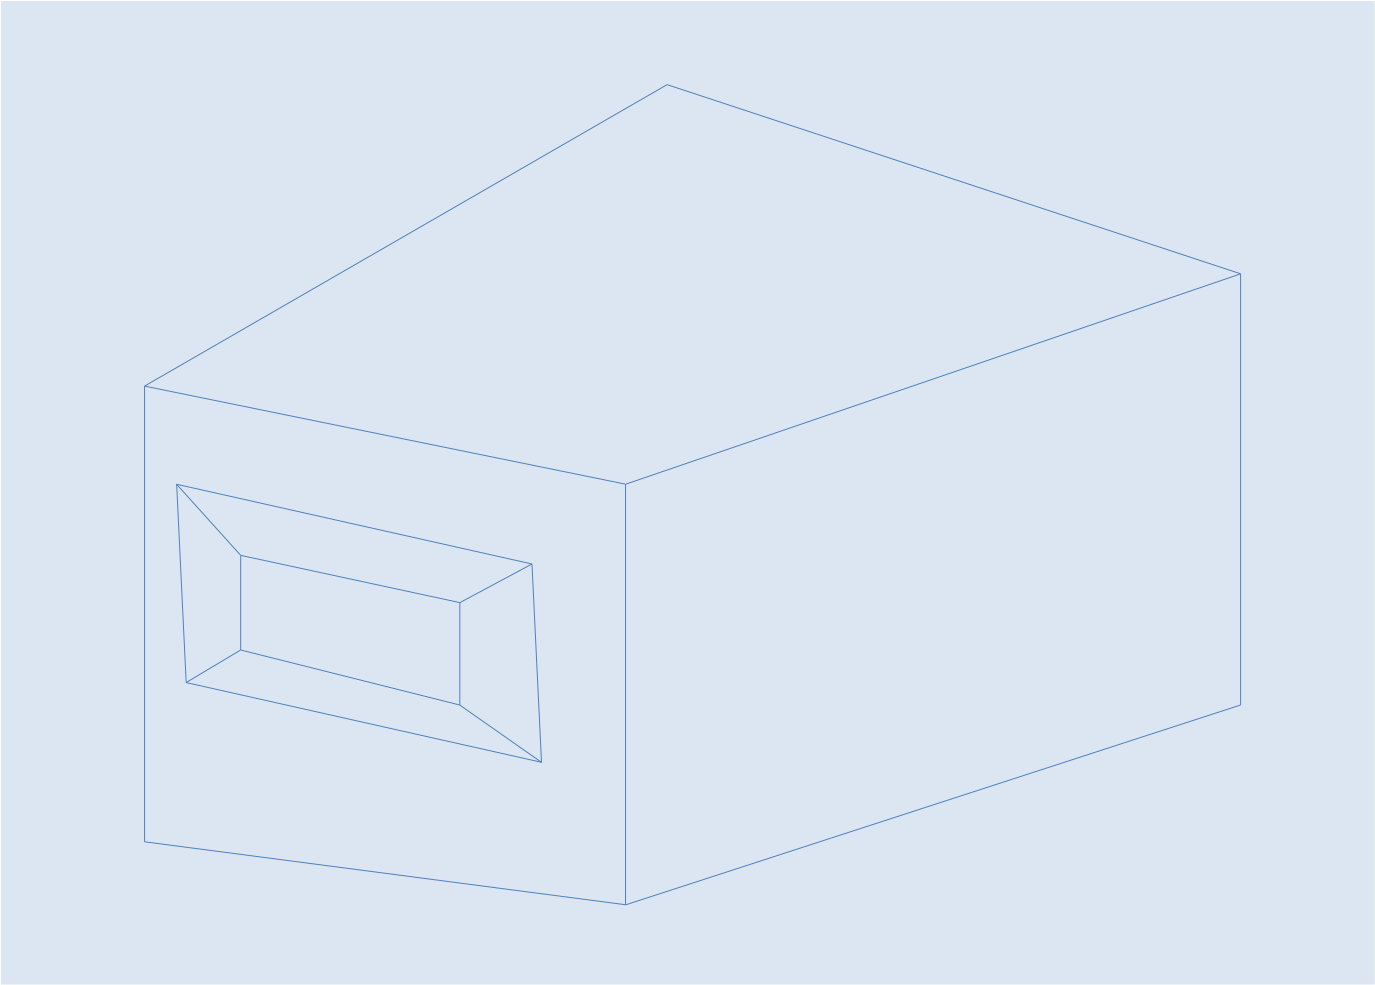
\includegraphics[width=60mm]{../image/sample6.png}
		\label{fig:sample5}}
	\caption{入力した画像}
	\label{fig:input}
\end{figure}


\subsection{写真画像の入力に依る実験}
撮影した画像を入力して解析を行った.入力した写真は,図\ref{fig:input_pic}に示した.

\begin{figure}[H]
\centering
	\subfigure[picture0]{
		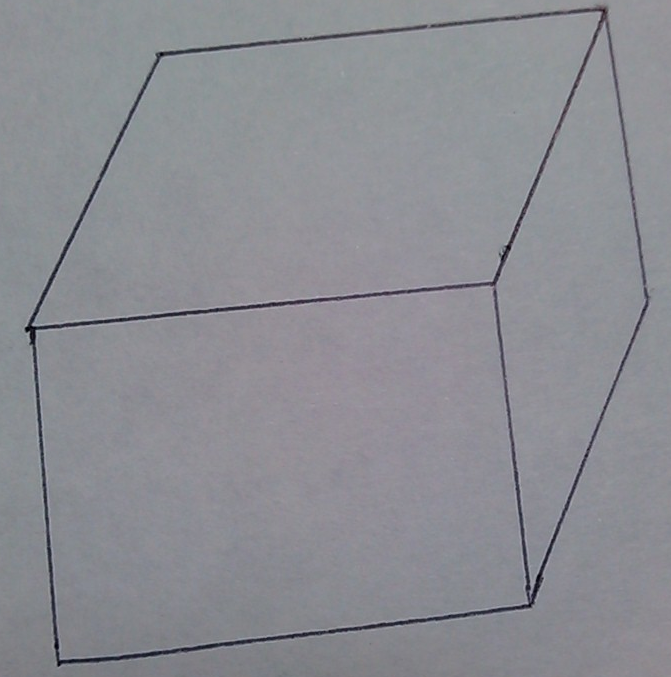
\includegraphics[width=50mm]{../image/pic0.png}
		\label{fig:pic0}}
	\subfigure[picture1]{
		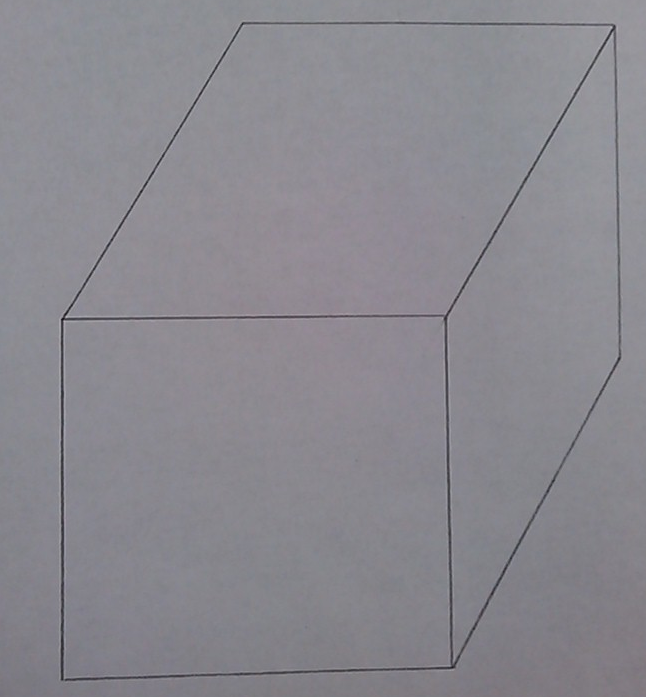
\includegraphics[width=50mm]{../image/pic1.png}
		\label{fig:pic1}}
	\subfigure[picture2]{
		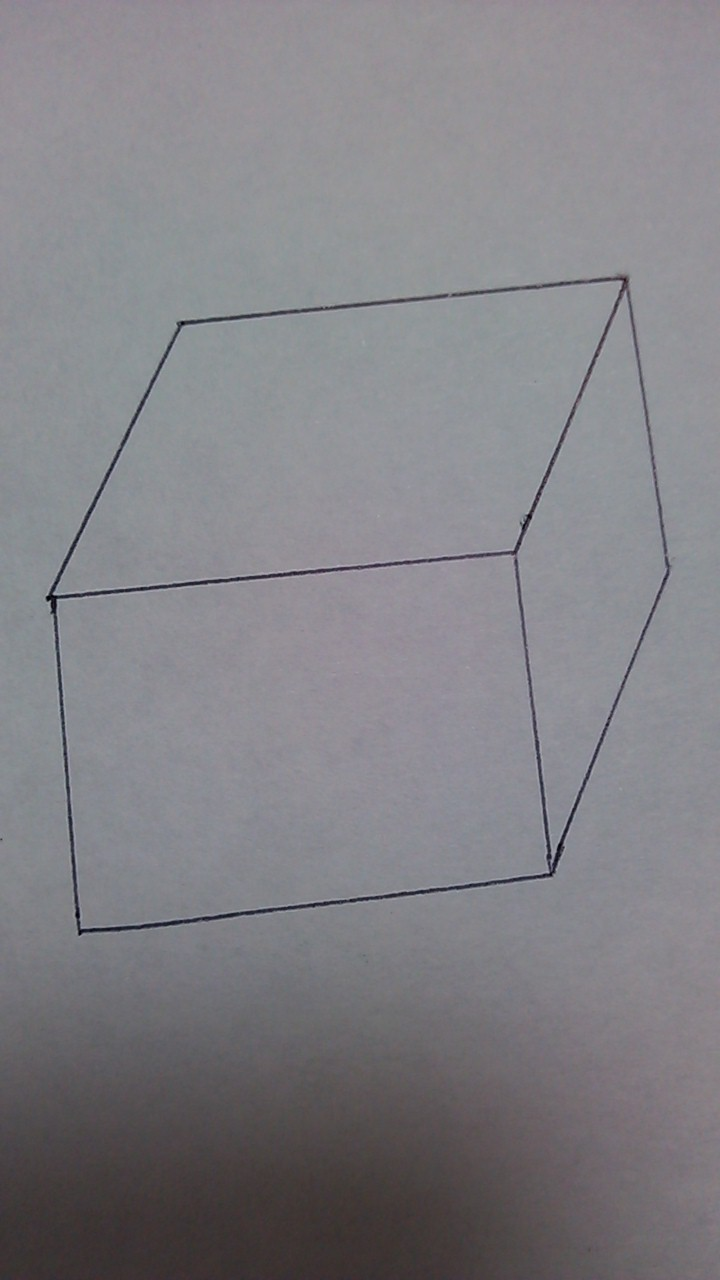
\includegraphics[width=50mm]{../image/pic2.jpg}
		\label{fig:pic2}}
	\caption{入力した写真画像}
	\label{fig:input_pic}
\end{figure}






%------
\section{実験結果}
\subsection{テキスト入力による実験の結果}
テキストを入力した結果を図\ref{fig:res_text}に示した.
\begin{figure}[H]
\begin{center}
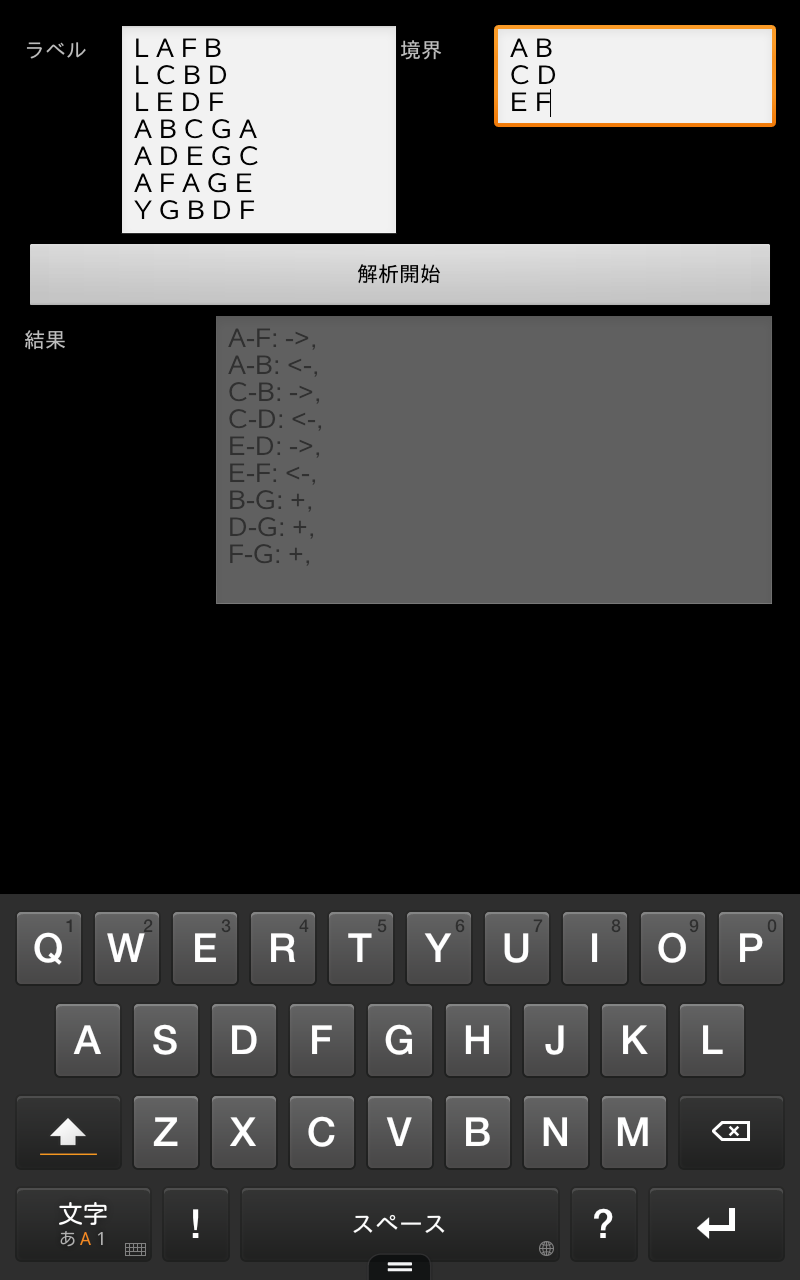
\includegraphics[width=65mm]{../play_store/text_analysis.png}
\caption{テキスト入力の結果}
\label{fig:res_text}
\end{center}
\end{figure}

出力結果を見ると,リスト\ref{code:text_analysis}のようになる.ただし,「A-F: $\rightarrow$」などは,AからFに矢印が向いているという意味になる.結果が一意に定まっているとわかる.
\lstset{style=customplain}
\lstinputlisting[caption=テキスト入力の結果, label=code:text_analysis]{source/res_text.txt}



\subsection{描画ソフトによる画像の入力に依る実験の結果}
描画ソフトによる画像を入力した結果を図\ref{fig:res_image}に示した.図\ref{fig:sample0_res}の図形と,図\ref{fig:example}の図形を見比べると,頂点の対応はずれて入るものの,前節のテキスト入力に依る実験の結果が正しいことがわかる.また,図\ref{fig:sample1_res}のように少しノイズがある図形も,特徴点抽出の閾値を調整することで正しく認識できるようになっている.

図\ref{fig:sample2_res}は不可能図形であるが,制約伝播アルゴリズムによって,「この図形は不可能図形です」と示されている.また,図\ref{fig:sample3_res}のネッカーキューブは,頂点DやFが4つの辺を持つために,「不可能図形であるか入力が不正です」と示されている.また,当初,4つの辺のときに,そのうちの3つの辺に対してのみ解釈をするようになっていた場合(条件の設定間違いをしていた)では,ネッカーキューブに対しても,いくつかの解の候補が表示された.

図\ref{fig:sample4_res}の図形は,本来は,内側に凹んでいる図形としても認識できる.しかし,この図形が浮いているものとみなし,境界の条件を決めたために,内側が盛り上がった図形として認識されている.一方で,図\ref{fig:sample5_res}では,図\ref{fig:sample4_res}の内側が凹んでいるか,盛り上がっているかの2通りの解釈ができるため,解の候補をテキストで表示している.

ただし,Androidでは画像の読み込みを個々の端末の解像度やメモリにあわせて調整するため,同じ結果が得られない場合があることがわかった.

\begin{figure}[H]
\centering
	\subfigure[sample0]{
		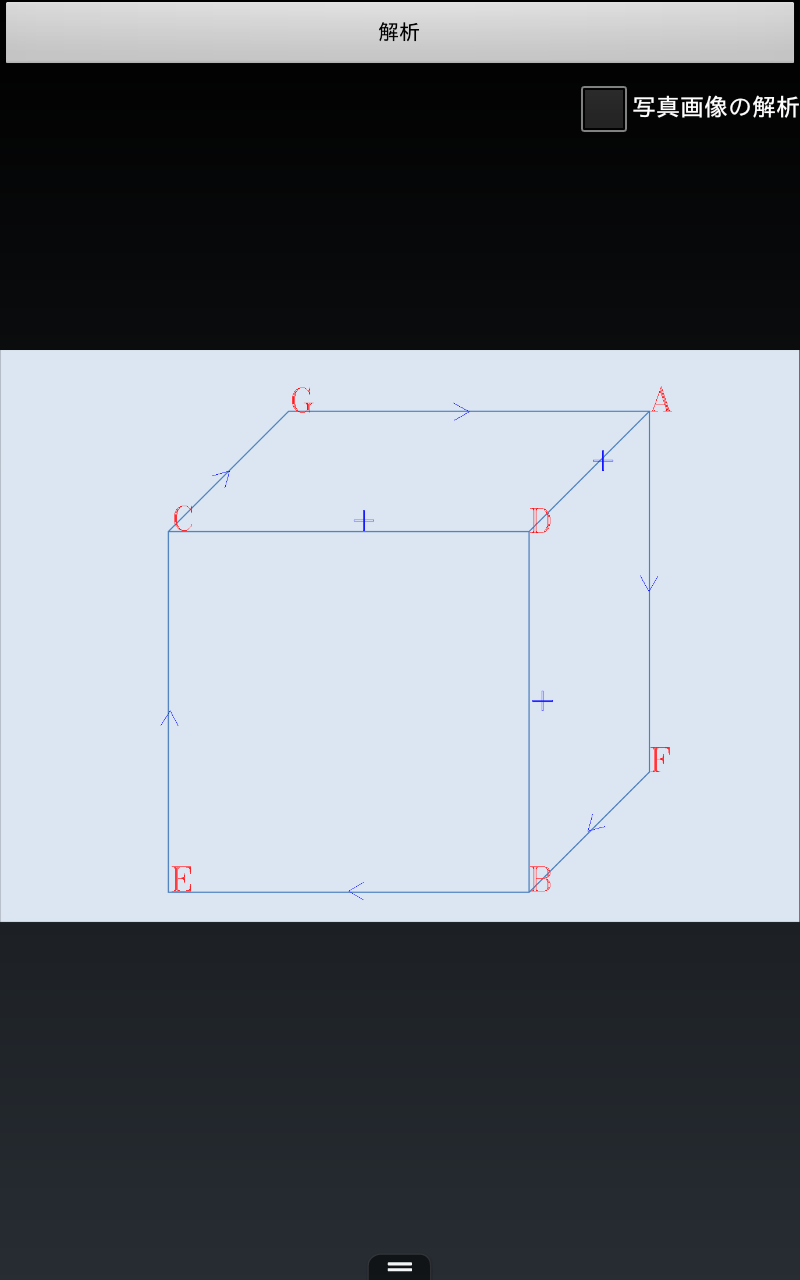
\includegraphics[width=60mm]{../play_store/sample0.png}
		\label{fig:sample0_res}}
	\subfigure[sample1]{
		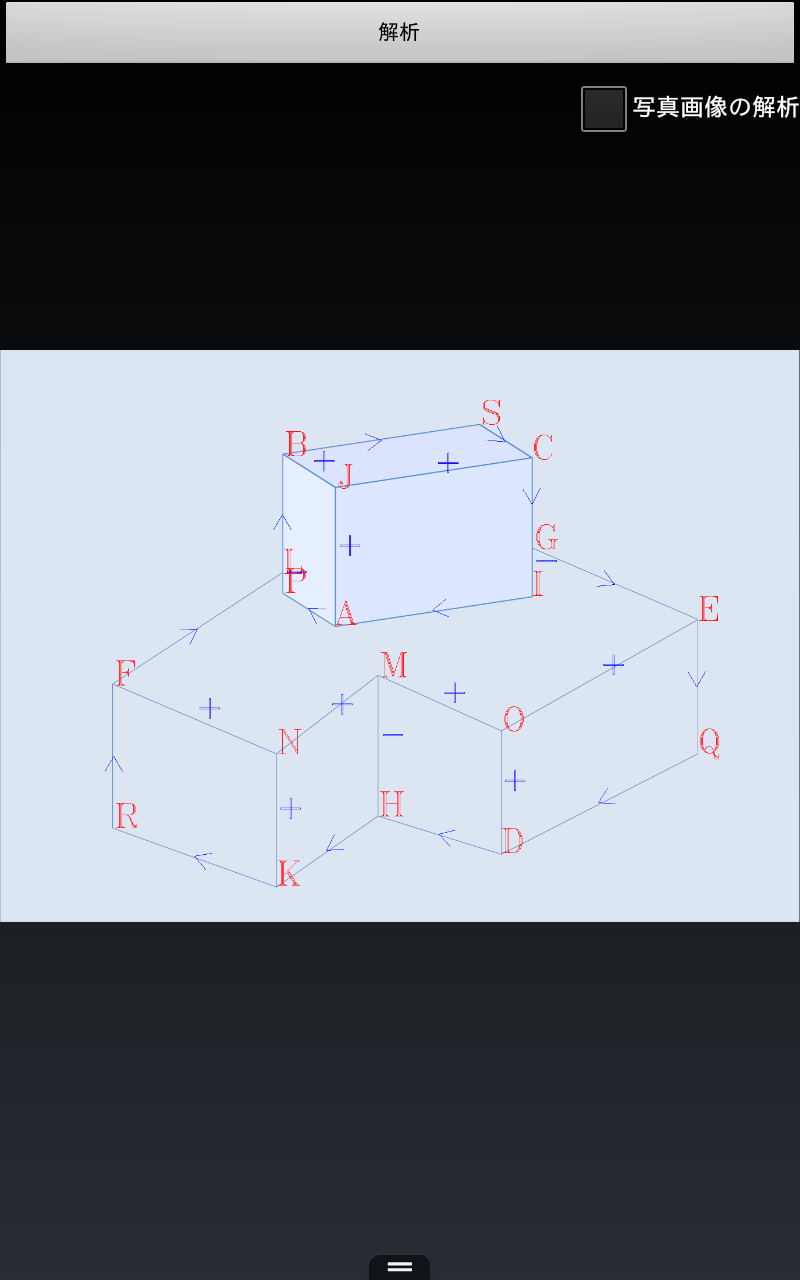
\includegraphics[width=60mm]{../play_store/sample2.png}
		\label{fig:sample1_res}}
	\subfigure[sample2]{
		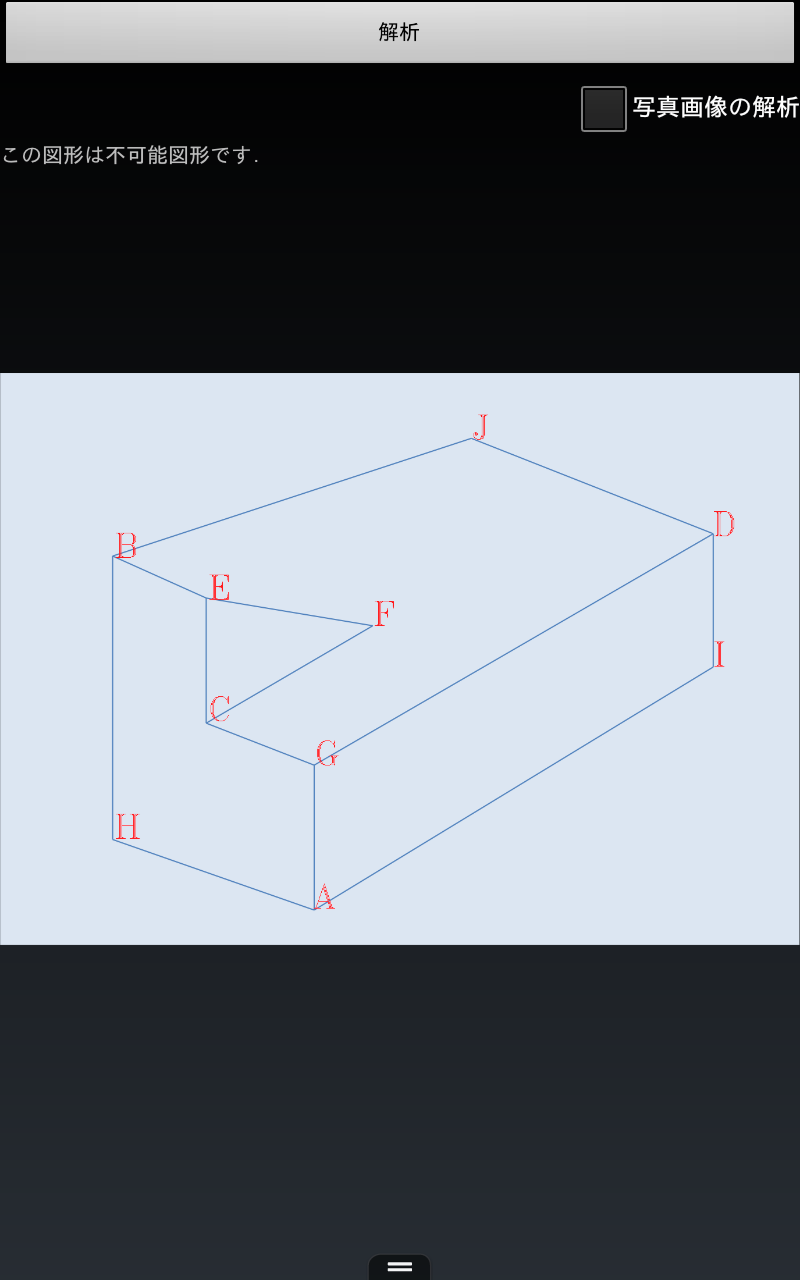
\includegraphics[width=60mm]{../play_store/sample3.png}
		\label{fig:sample2_res}}
	\subfigure[sample3]{
		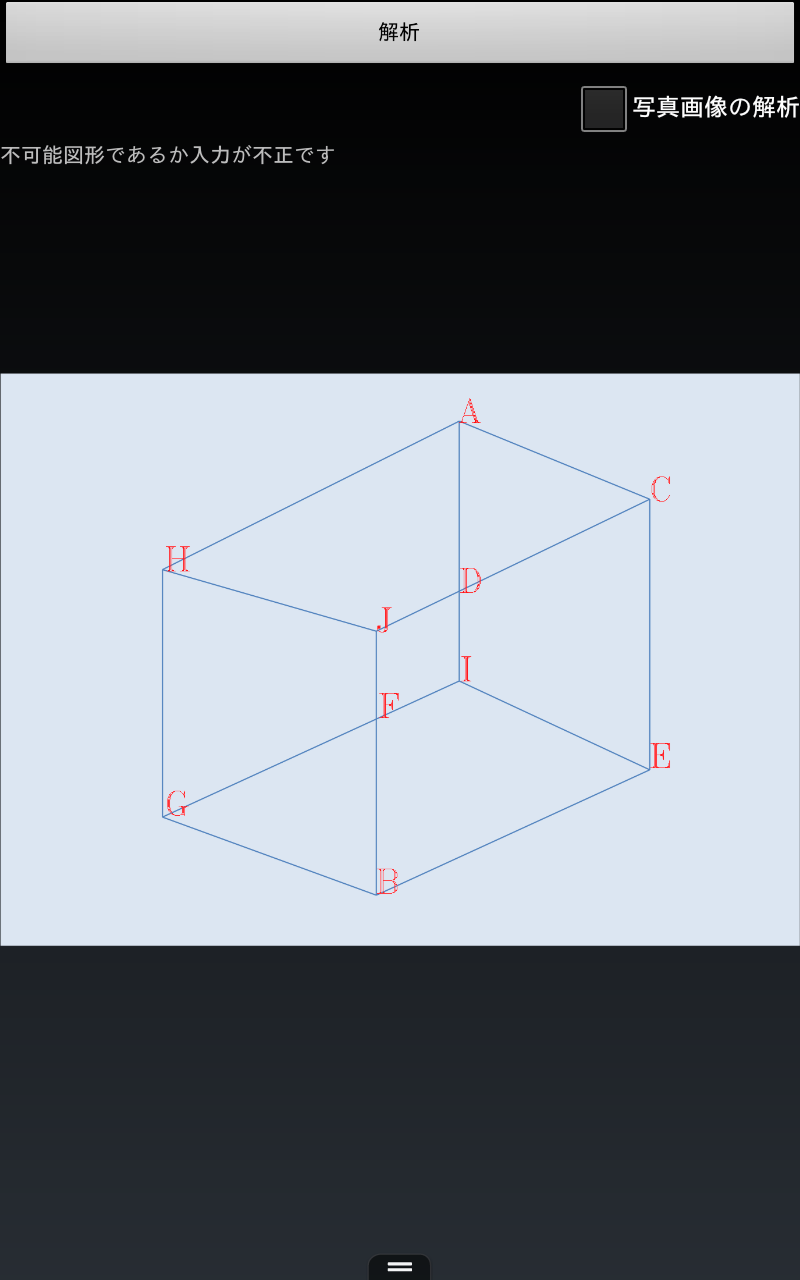
\includegraphics[width=60mm]{../play_store/sample4.png}
		\label{fig:sample3_res}}
	\subfigure[sample4]{
		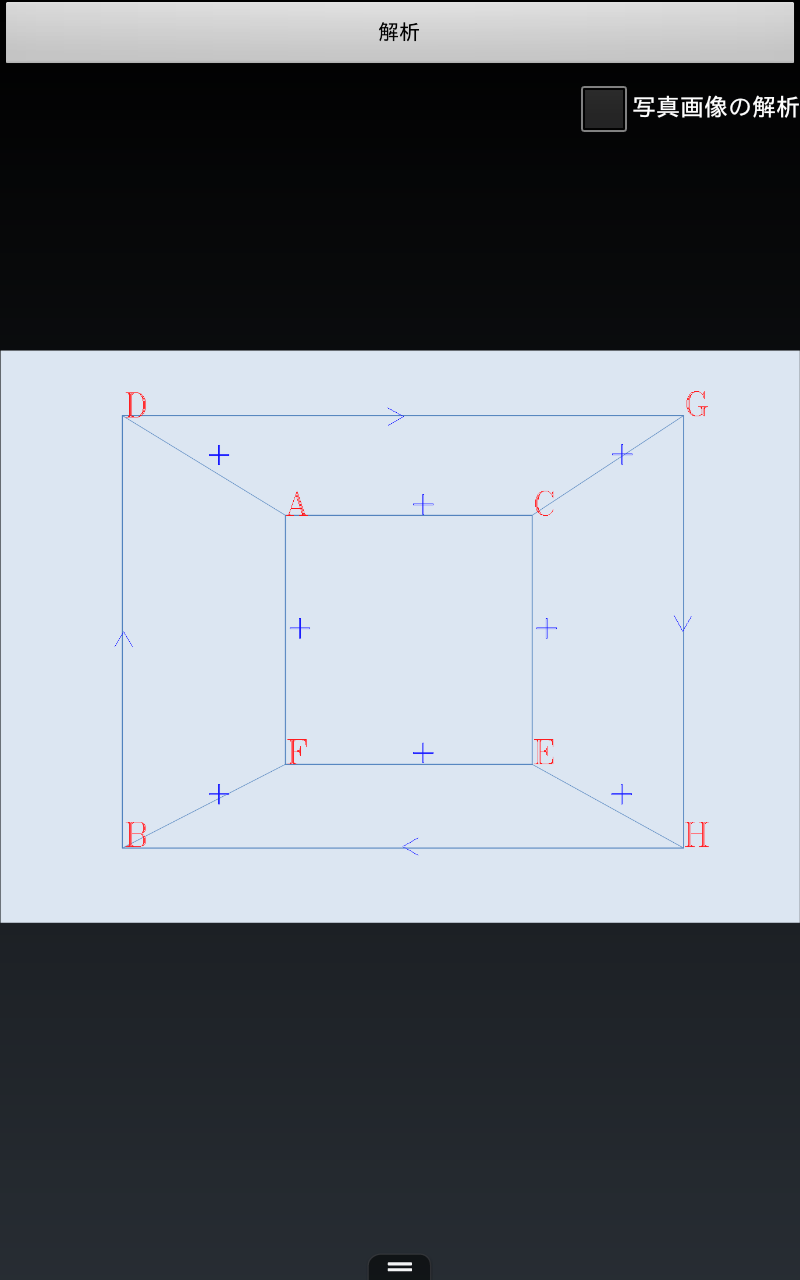
\includegraphics[width=60mm]{../play_store/sample5.png}
		\label{fig:sample4_res}}
	\subfigure[sample5]{
		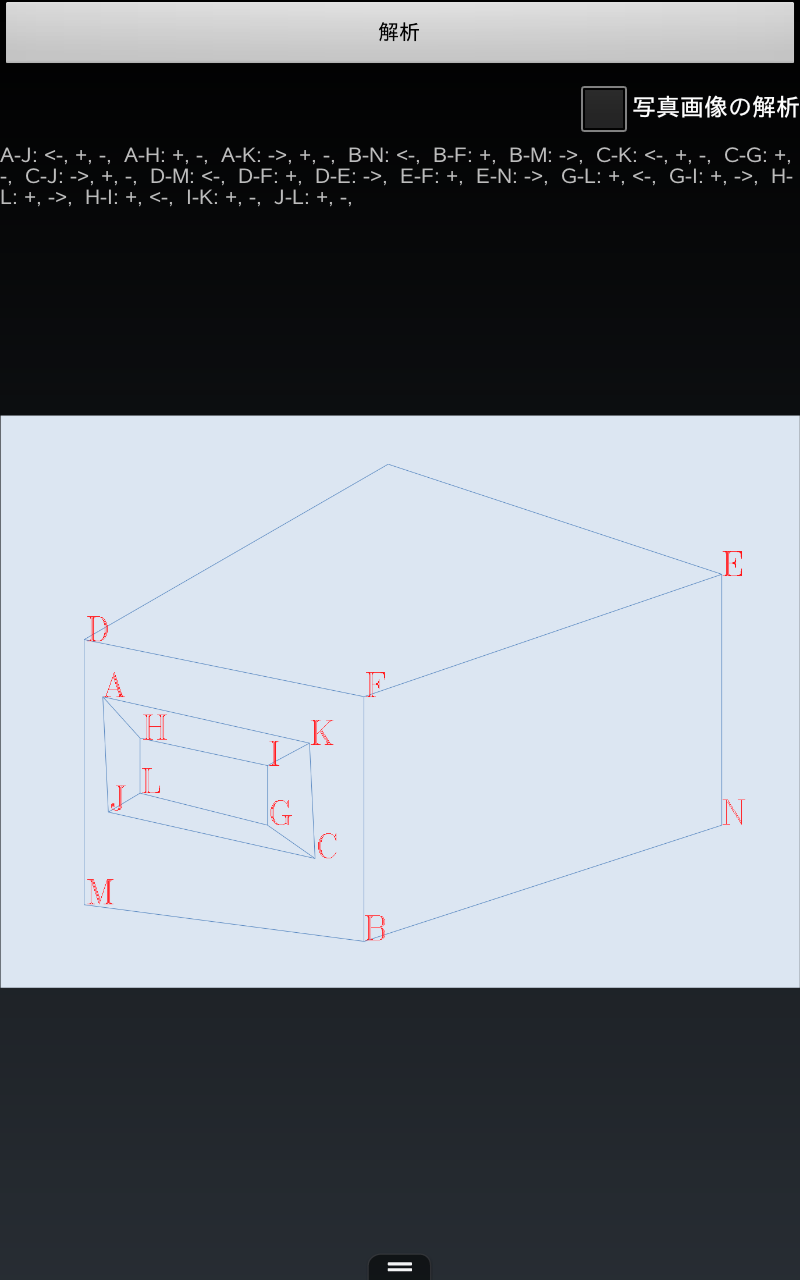
\includegraphics[width=60mm]{../play_store/sample6.png}
		\label{fig:sample5_res}}
	\caption{入力した画像の解釈結果}
	\label{fig:res_image}
\end{figure}



\subsection{写真画像の入力に依る実験の結果}
写真画像を入力した結果を図\ref{fig:res_pic}に示した.picture0とpicture1は下処理を行った場合と,行ってない場合の両方を示した.図\ref{fig:pic0_non_res}と図\ref{fig:pic0_res}を見比べると,特徴点抽出がわずかながら向上している事がわかる.しかし,元の画像で厚みがあった部分や曲がった部分などで特徴点が検出されてしまっている.

図\ref{fig:pic1_non_res}と図\ref{fig:pic1_res}を見比べると,下処理によって,斜めに検出されていた特徴点が全く検出されなくなり向上しているが,下処理の前にはなかった横向きの線に対して,特徴点が検出されてしまっているため正しく動作していない.

さらに,図\ref{fig:pic2_res}に関しては,影に特徴点が集中し,結果の出力に20秒程度の時間がかかった.

\begin{figure}[H]
\centering
	\subfigure[picture0に下処理を行わなかった場合]{
		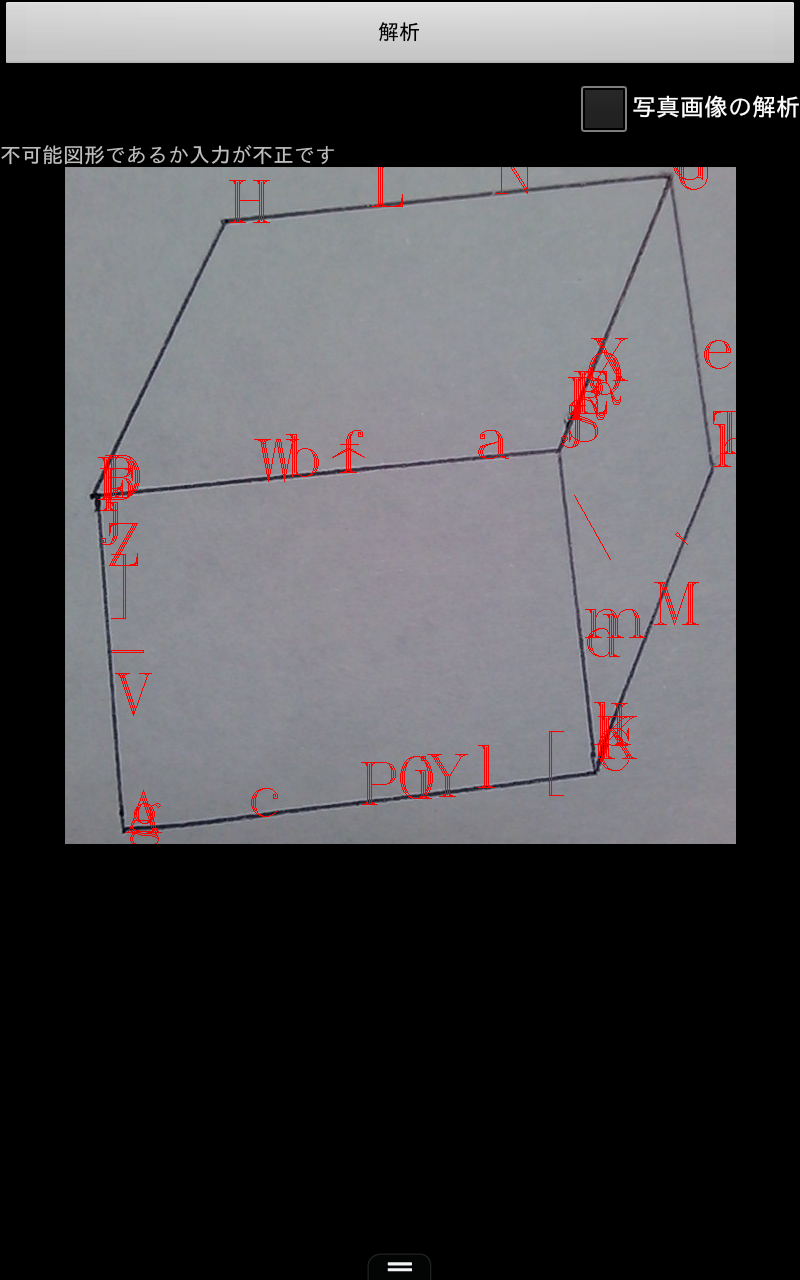
\includegraphics[width=60mm]{../play_store/pic0_non.png}
		\label{fig:pic0_non_res}}
	\subfigure[picture0に下処理を行った場合]{
		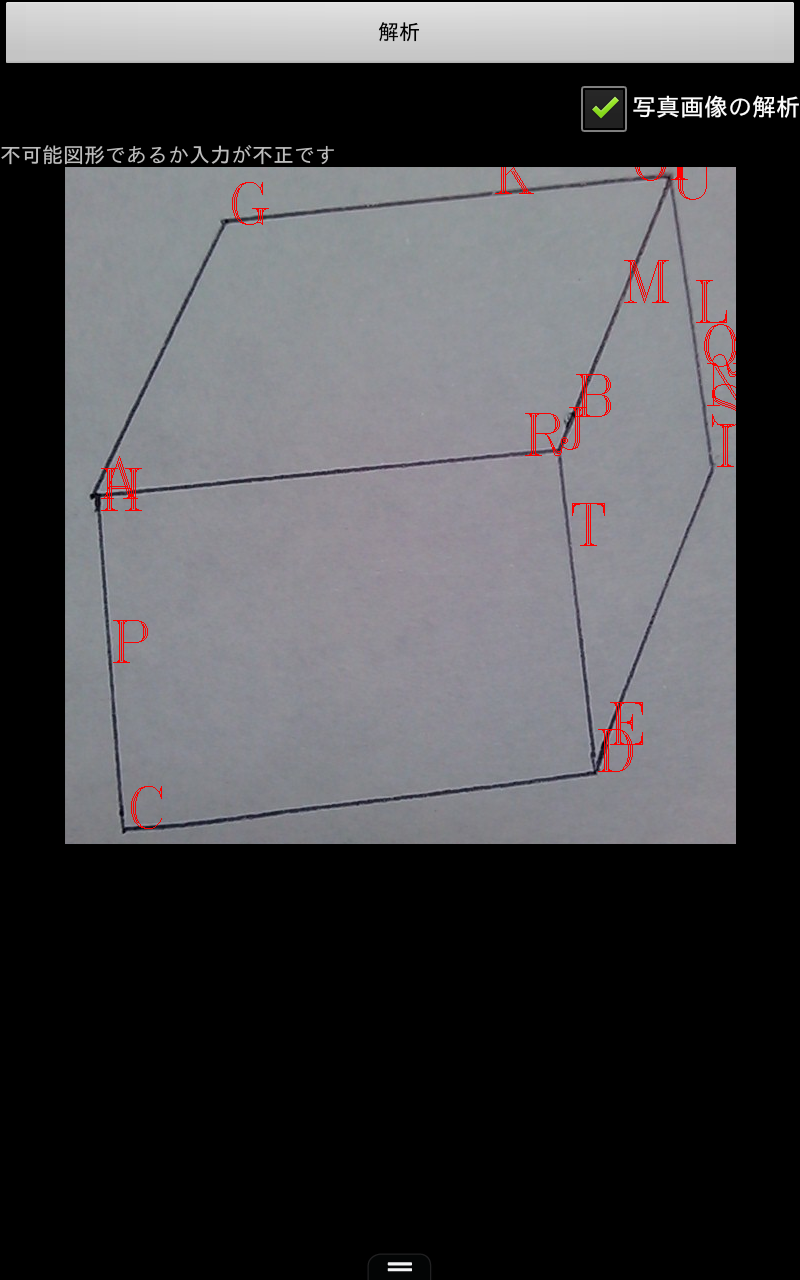
\includegraphics[width=60mm]{../play_store/pic0.png}
		\label{fig:pic0_res}}
	\subfigure[picture1に下処理を行わなかった場合]{
		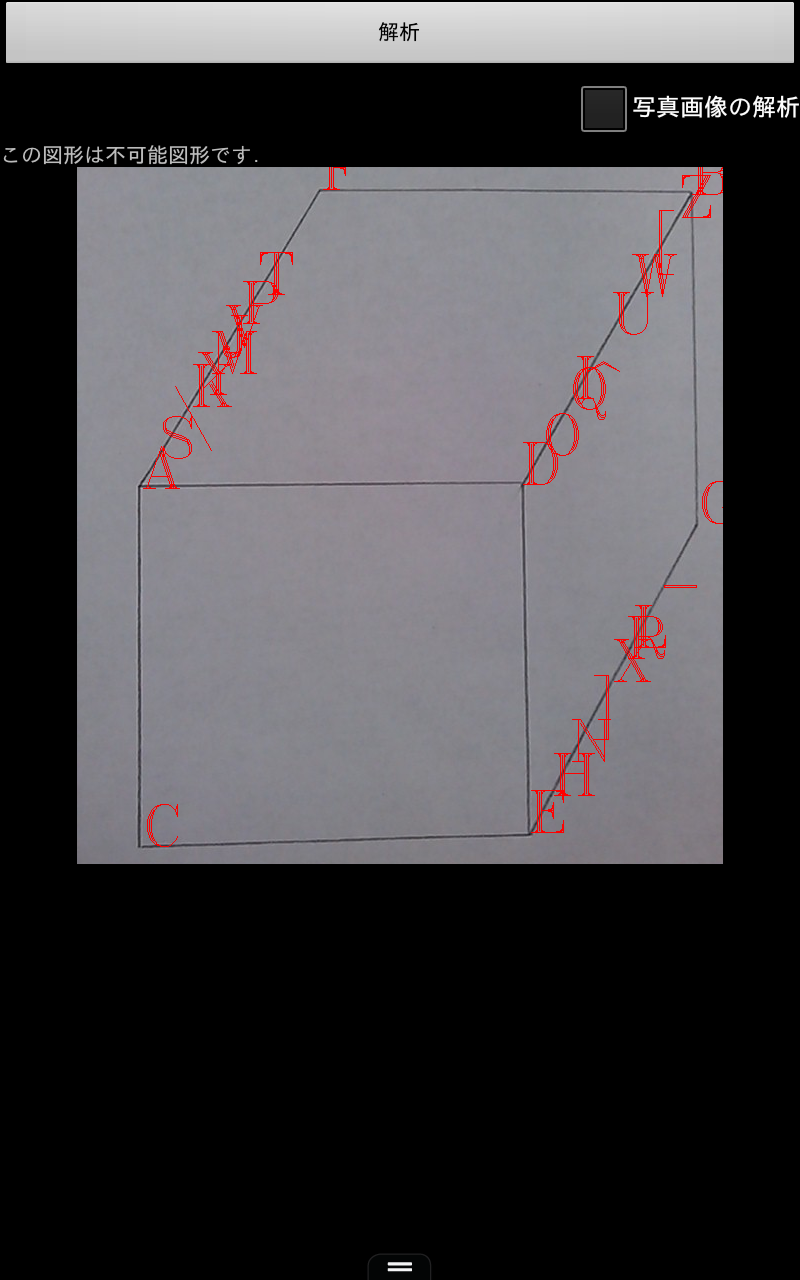
\includegraphics[width=60mm]{../play_store/pic1_non.png}
		\label{fig:pic1_non_res}}
	\subfigure[picture1に下処理を行った場合]{
		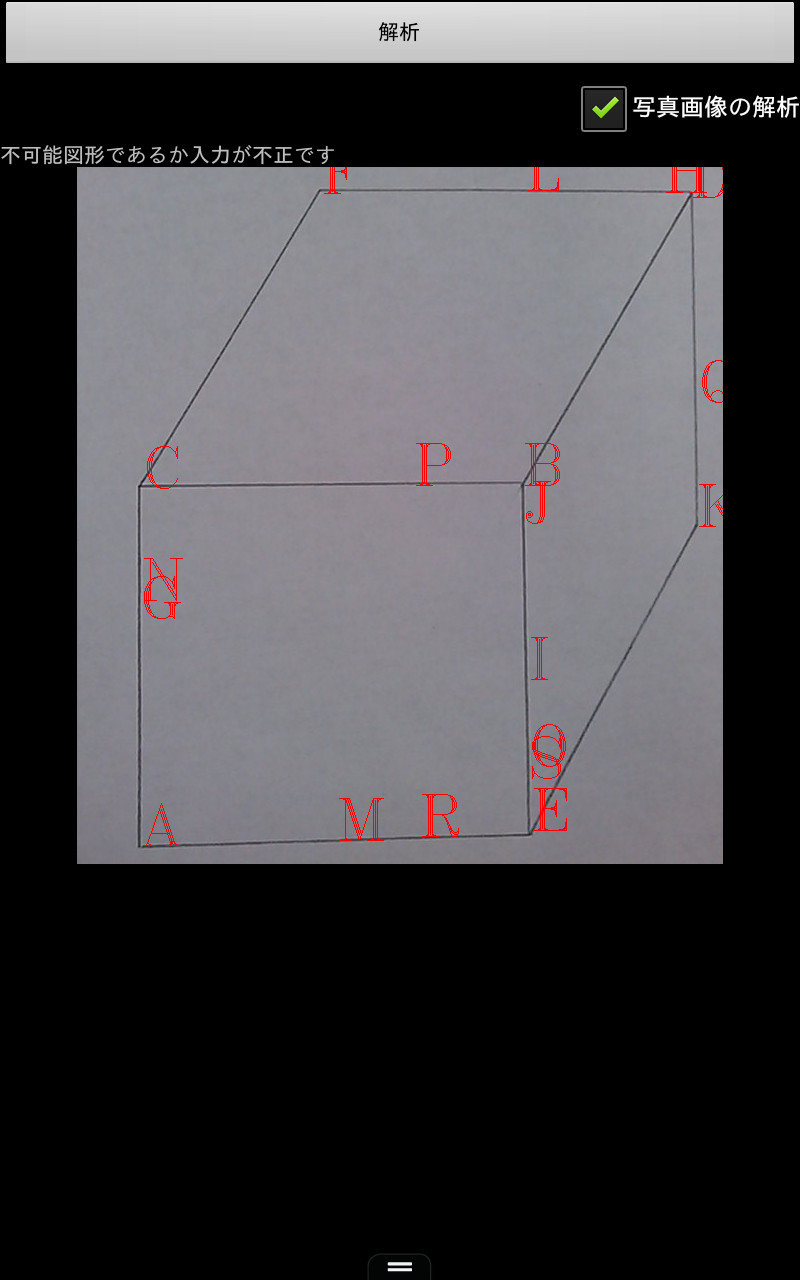
\includegraphics[width=60mm]{../play_store/pic1.png}
		\label{fig:pic1_res}}
	\subfigure[picture2に下処理を行った場合]{
		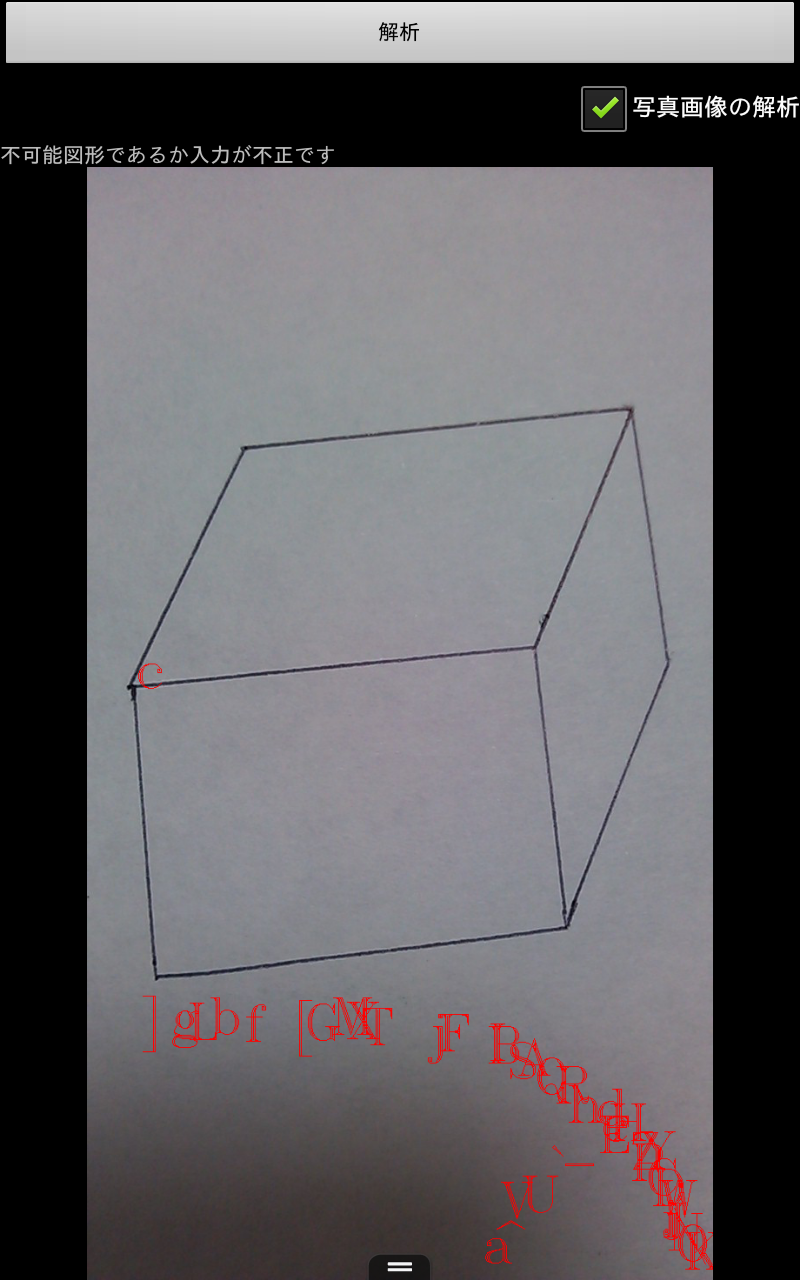
\includegraphics[width=60mm]{../play_store/pic2.png}
		\label{fig:pic2_res}}
	\caption{入力した写真画像の解釈結果}
	\label{fig:res_pic}
\end{figure}






%------
\section{考察}
\subsection{テキスト入力による実験の考察}
テキスト入力に対する結果と,画像による入力結果,参考文献\cite{ref:labeling}をあわせて考えると,テキスト入力による解釈は正しく動作していると考えられる.しかし,今回のアルゴリズムでは,解が一意に定まらなかった場合に,頂点と辺によって候補を絞っていくだけであったため,全体としてみればそれぞれの制約条件から結果が一意に定まる場合を考慮できていない.

複雑な図形でも,頂点情報を正しく入力できれば正しい結果が得られると推察される.



\subsection{描画ソフトによる画像の入力に依る実験の考察}
描画ソフトに依る画像の入力に対しては,実験結果から正しく動作することがわかる.ただし,Androidでは画像の読み込みを個々の端末の解像度やメモリにあわせて調整するため,同じ結果が得られない場合があることがわかった.これに対しては,写真画像と同様にした処理を行ってから画像を入力することで解決できると考えられる.

ただし,テストした環境では正しく解釈されたことが結果からわかる.特に図\ref{fig:sample1_res}のような複雑な図形に対しても解釈が行えている.この図は,当初,上部の図形が滑らかでなかったために,特徴点が角でないところで検出されるなどの問題があったが,経験から設定した閾値によって,正しく解釈されるようになっている.

また,不可能図形に対しても,その旨が表示できており,アルゴリズムが正しく動作されていることがわかる.一方,ネッカーキューブのような図では,結果でも触れたように,接続している辺が3つよりも多くても,そのうちの3つに対して処理を行うと,解釈の候補が幾つか表示された.本来,このような処理にならないようにするべきで,結果に示したように「不可能図形であるか入力が不正です」と表示されるべきであった.この失敗から得られた結果について考えてみる.この結果を,図\ref{fig:necker}に示した.

\begin{figure}[H]
\begin{center}
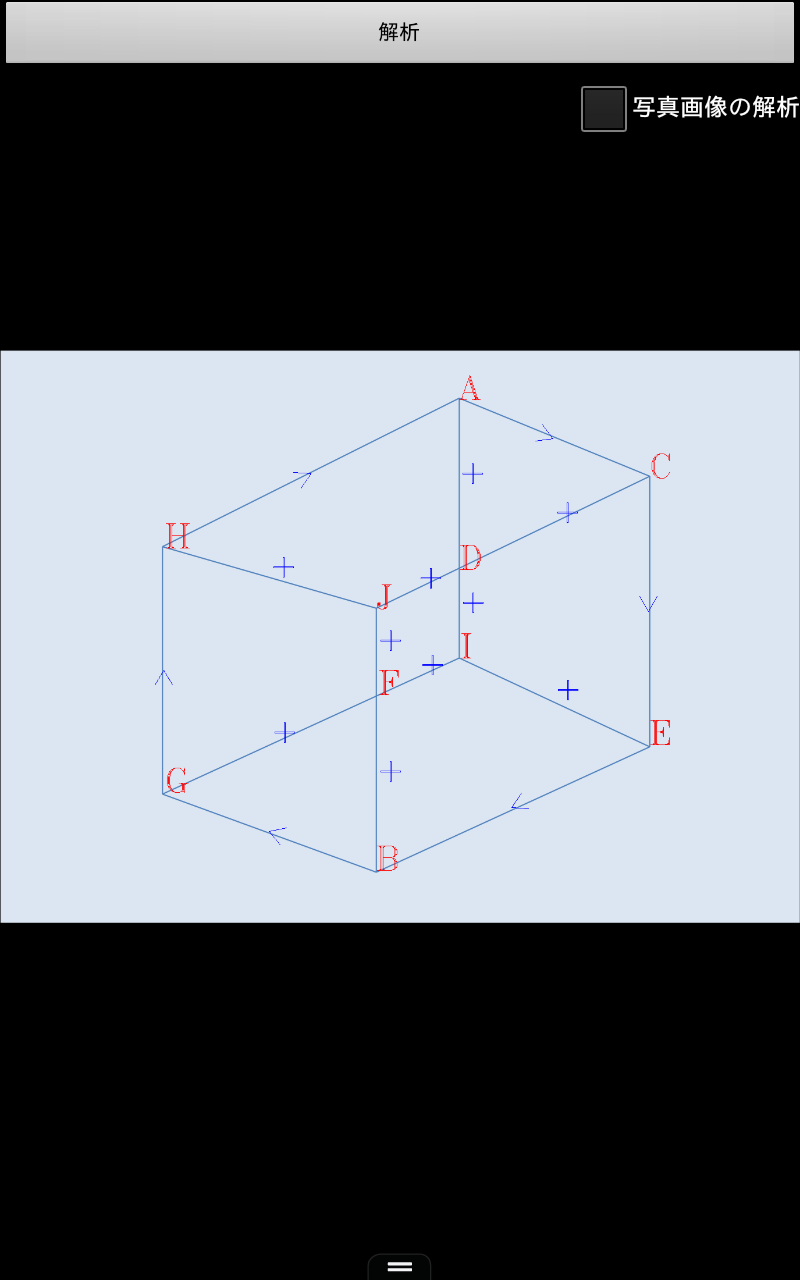
\includegraphics[width=65mm]{../play_store/necker.png}
\caption{ネッカーキューブの解釈}
\label{fig:necker}
\end{center}
\end{figure}

この結果から,辺AI,EI,GIによる角と,辺HJ,CJ,BJによる角のどちらもが飛び出して見えていることがわかる.これは,図\ref{fig:sample4_res}のように境界による条件で,内側が飛び出した図形と判断されるためと推察される.つまり,このアルゴリズムでは,人間と同様にどちらの角も飛び出しているように解釈できるというわけである.また,境界の条件をなくせば,内側が凹んでいる図形と解釈されることが図\ref{fig:sample5_res}の結果から推察される.このことを反対にアルゴリズムの視点から捉えると,人間はこのようなどちらの解釈もできる図形に対して,同様のアルゴリズムにしたがって解釈を行っている可能性が考えられる.

また,画像からの解釈でもテキスト入力の際に用いた解析器を用いているため,正しく動作していることからテキスト入力による解釈の正しさも示された.



\subsection{写真画像の入力に依る実験の考察}
写真画像の入力による実験では,正しい結果が得られなかった.その原因は,実験に使用した図から,
\begin{itemize}
	\item 細線化の際にエイリアシングを作ってしまっている
	\item 影が図形として解釈される
	\item 線に膨らみがある場合,細線化を行うとよりそれが際立ってしまう
\end{itemize}
などが挙げられるとわかる.一方で,細線化とsmoothingによって,無駄な特徴点が検出されないように改善されている図もあり,方針としては正しいと考える.現在は直線近似によって,線を滑らかにし,そこから角を検出しているが,あらかじめ角の検出に特化したアルゴリズムを用いて角を正確に抽出できれば,それらをつなぐことでよりなめらかな線図を出力できると推察される.



% -----
\section{結論}
本課題では,テキストや画像からの線画解析を試みた.その結果,テキスト入力に関しては正しい結果を返し,画像でもノイズの少ないもの解釈であれば,正常に処理を行えることが確認できた.ただし,写真からの認識は,線画へと下処理をする部分で,画像処理による知識が乏しく,正しく認識することが出来ないという結果になってしまったことが反省としてあげられる.提出締め切りまでさらに検討してみようと考えている.

それらの手法では,OpenCVという画像処理ライブラリに依る部分が多く,初めて使用したものの,その便利さがよくわかった.また,アルゴリズムでは,参考文献\cite{ref:labeling}の通りに実装することで実現ができた.他の参考文献からも,様々な情報を得ることが出来た.感謝を示したい.




\begin{thebibliography}{n}
\bibitem{ref:labeling}
『レポート課題:「制約伝播:線画のラベリング」資料』,\url{http://www.slis.tsukuba.ac.jp/~hiraga.yuzuru.gf/AI/label.shtml}

\bibitem{ref:opencv_honke}
『OpenCV』,\url{http://opencv.org/}

\bibitem{ref:opecv_manager}
『Google Play - OpenCV Manager』,\url{https://play.google.com/store/apps/details?id=org.opencv.engine&hl=ja}

\bibitem{ref:dropbox}
『DropBox』,\url{https://www.dropbox.com/login?lhs_type=anywhere}

\bibitem{ref:file_transfer}
『Android File Transfer』,\url{http://android-file-transfer.softonic.jp/mac}

\bibitem{ref:astro}
『アストロファイルマネージャー』,\url{https://play.google.com/store/apps/details?id=com.metago.astro&hl=ja}

\bibitem{ref:android_dev}
『Mac(OS X Mountain Lion)にAndroidの開発環境を構築』,\url{http://blog.wadous.com/it/android/424.html}

\bibitem{ref:opencv_android}
『OpenCV for android 2.4.3』,\url{http://d.hatena.ne.jp/Kazzz/20121128/p1}

\bibitem{ref:file_explorer}
『【Android】ファイル選択ダイアログを作成』,\url{http://alldaysyu-ya.blogspot.jp/2013/09/android_12.html}

\bibitem{ref:opencv_api}
『OpenCV.jp』,\url{http://opencv.jp/}

\bibitem{ref:thinning}
『細線化』,\url{http://www.eml.ele.cst.nihon-u.ac.jp/~momma/wiki/wiki.cgi/OpenCV/%E7%B4%B0%E7%B7%9A%E5%8C%96.html#h7}

\bibitem{ref:harris}
『cagylogic』,\url{http://www.cagylogic.com/archives/2009/03/03000100.php}

\bibitem{ref:outer}
『基礎の基礎編 その1 内積と外積の使い方』,\url{http://marupeke296.com/COL_Basic_No1_InnerAndOuterProduct.html}

\bibitem{ref:book}
伊庭 斉志 :『人工知能と人工生命の基礎』,オーム社 (2013.5.24)


\end{thebibliography}

\end{document}












